% \documentclass{article}
\documentclass[journal=jpclcd,manuscript=article]{achemso}
\usepackage[utf8]{inputenc}

% ALL: See "style guide" here: % https://docs.google.com/document/d/12xwId6RT73miifI1thtLL7c0GoVIXsSfZndO5bgdqag/edit#

% Tables
% Use Roman numerals for tables
% https://tex.stackexchange.com/a/226029
\usepackage[labelsep=period]{caption}
\captionsetup[table]{name=Table}
\renewcommand{\thetable}{\Roman{table}}
% \usepackage{multirow}

\usepackage{pdflscape}
\usepackage{textcomp}
\usepackage{gensymb}
\usepackage{geometry}

\usepackage{subcaption} % For subfigures?

\usepackage{pifont}
\newcommand{\cmark}{\textcolor{blue}{\textrm{\ding{52}}}}%
\newcommand{\xmark}{\textcolor{red}{\textrm{\ding{56}}}}%

\usepackage{amsmath}
\usepackage{amssymb}
%usepackage{authblk}


% units
% \SI{X}{\UNIT} will write the value X with units \UNIT. 
% eg. \SI{30}{\celsius}
\usepackage{siunitx} 

\usepackage{graphicx}
\graphicspath{ {./images/} }

\setlength {\marginparwidth }{2cm}
\usepackage{todonotes}
\newcommand{\tino}[1]{\todo[inline,color=purple!40]{Tino: #1}}
\newcommand{\fbp}[1]{\todo[inline,color=orange!40]{Ferran: #1}}
\newcommand{\summary}[1]{\todo[inline,caption={},color=yellow!40]{Summary: \\ #1}}

\newcommand{\ssri}[1]{{
\fbox{
\parbox{0.8\textwidth}{  \fbox{$\triangleright$\textcolor{blue}{\textbf{Shashank}:}} 
#1
}}}}

\newcommand{\gbox}[1]{{
\fbox{
\parbox{0.8\textwidth}{  \fbox{$\triangleright$\textcolor{blue}{\textbf{Gon}:}} 
#1
}}}}

\newcommand{\pbox}[1]{{
\fbox{
\parbox{0.8\textwidth}{  \fbox{$\triangleright$\textcolor{blue}{\textbf{From Peter}:}} 
#1
}}}}

\newcommand{\pdebox}[1]{{
\fbox{
\parbox{0.8\textwidth}{  \fbox{$\triangleright$\textcolor{blue}{\textbf{From Philipp}:}} 
#1
}}}}

\newcommand{\editreadybox}[1]{{
\fbox{
\parbox{0.8\textwidth}{  \fbox{$\triangleright$\textcolor{green}{\textbf{READY TO EDIT}:}} 
#1
}}}}

\usepackage[normalem]{ulem}

\setlength{\textheight}{8.4in}
\setlength{\topmargin}{0.1in}
\setlength{\headheight}{0.2in}
\setlength{\headsep}{0.1in}
\setlength{\oddsidemargin}{0in}
\setlength{\textwidth}{6.5in}

\title{``Knees'' in lithium-ion battery aging trajectories}


\author{Peter M. Attia}
\email{peter.m.attia@gmail.com}
\affiliation{Department of Materials Science and Engineering, Stanford University, Stanford, California, USA}
\author{Alexander Bills} 
\affiliation{Department of Mechanical Engineering, Carnegie Mellon University, Pittsburgh, PA, USA}
\author{Ferran Brosa Planella} 
\affiliation{WMG, University of Warwick, Coventry, CV4 7AL, UK, and Faraday Institution, Harwell, UK}
\author{Philipp Dechent} 
\affiliation{Institute for Power Electronics and Electrical Drives (ISEA), RWTH Aachen University, 52066 Aachen, Germany}
%%%%%%%%%%%%%%%%%%%%%%%%%%%%%%%%%%%%%%%%%%%%%%%%%%%%%%%%
\author{Gon\c{c}alo dos Reis} 
% Goncalo's ORCID: 0000-0002-4993-2672
\affiliation{School of Mathematics, University of Edinburgh, The King’s Buildings, Edinburgh, EH9 3FD, UK}
\affiliation{Centro de Matem\'atica e Aplica\c c$\tilde{\text{o}}$es (CMA), FCT, UNL, Quinta da Torre, 2829-516 Caparica, Portugal}
%%%%%%%%%%%%%%%%%%%%%%%%%%%%%%%%%%%%%%%%%%%%%%%%%%%%%%%%
\author{Matthieu Dubarry}
\affiliation{Hawaii Natural Energy Institute, University of Hawaii, Honolulu, HI, USA}
\author{Paul Gasper} 
\affiliation{National Renewable Energy Laboratory, 15013 Denver West Pkwy, Golden, CO, USA}
\author{Samuel Greenbank} 
\affiliation{Department of Engineering Science, University of Oxford, Parks Road, Oxford, OX1 3PJ, United Kingdom, and Faraday Institution, Harwell, UK}
\author{David Howey} 
\affiliation{Department of Engineering Science, University of Oxford, Parks Road, Oxford, OX1 3PJ, UK, and Faraday Institution, Harwell, UK}
\author{Ouyang Liu} 
\affiliation{Institute for Infocomm Research, Agency for Science, Technology, and Research (A*STAR), 1 Fusionopiationolis Way, Connexis, Singapore}
\author{Edwin Khoo}  
\affiliation{Institute for Infocomm Research, Agency for Science, Technology, and Research (A*STAR), 1 Fusionopiationolis Way, Connexis, Singapore}
\author{Yuliya Preger}  
\affiliation{Sandia National Laboratories, 1515 Eubank Blvd SE, Albuquerque, NM, USA}
\author{Abhishek Soni}
\affiliation{Please insert affiliation here Abhishek}
\author{Shashank Sripad} 
\affiliation{Department of Mechanical Engineering, Carnegie Mellon University, Pittsburgh, PA, USA}
\author{Anna G. Stefanopoulou}  
\affiliation{University of Michigan, Ann Arbor, MI, USA}
\author{Valentin Sulzer}
\affiliation{University of Michigan, Ann Arbor, MI, USA}



\date{}

\begin{document}
\maketitle

%**PREVIOUS DRAFT IS NOW IN main\_old\_experiment\_then\_model.tex**

\section{Abstract}

\pbox{To do}

Lithium-ion batteries can last many years but can exhibit 

In this work, we review prior work on ``knees'' in lithium-ion battery aging trajectories.
We first discuss
We then outline six knee ``pathways'', including 
Our findings illustrate the complexity and subtleties of lithium-ion battery degradation.

\newpage

Lithium-ion batteries will continue to play a critical role in decarbonization via their use in electric vehicle and stationary energy storage applications. One of the most challenging requirements for these demanding applications is long lifetime, with typical warranties of 8 years for electric vehicles and 10 years for grid storage.\cite{hesse_lithium-ion_2017, bocca_optimal_2020, beltran_lifetime_2020} Battery lifetime requirements will only become more demanding as “million-mile batteries”\cite{harlow_wide_2019} become the expectation for next-generation electric vehicles. Furthermore, as concerns around battery materials mining, manufacturing, and disposal increase, improving battery lifetime is a straightforward way to reduce the environmental impact of the lithium-ion battery lifecycle. Thus, understanding and improving the lifetime of lithium-ion batteries is a critical research direction.

Lithium ion batteries often exhibit either linear, sublinear, or superlinear aging trajectories (Figure \ref{fig:degradation_shapes}). In laboratory settings (i.e., single-cell testing using battery cyclers), these aging trajectories are typically presented as capacity or energy vs. cycle number or equivalent full cycles (EFCs). Aging trajectories are often linear[] or sublinear\cite{bloom_accelerated_2001, broussely_aging_2001, wright_calendar-_2002, smith_high_2011, attia_revisiting_2020}. Sublinear degradation is often attributed to side reactions such as solid-electrolyte interphase (SEI) growth, which grows approximately\cite{bloom_accelerated_2001, broussely_aging_2001, wright_calendar-_2002, smith_high_2011} (but not exactly\cite{attia_revisiting_2020}) with the square root of time or cycle number due to its self-passivating nature. While this type of degradation is largely unavoidable, the decelerating degradation rate is a fortunate property for long-lifetime applications. However, superlinear battery degradation is also observed (Figure \ref{fig:degradation_shapes}c). This type of degradation goes by many names in the battery literature, including ``knee''(cite), ``rollover failure''\cite{ma_editors_2019}, ``accelerated aging'', ``nonlinear aging''\cite{schuster_nonlinear_2015, bach_nonlinear_2016, yang_modeling_2017, mandli_analysis_2019, keil_linear_2019, atalay_theory_2020}, ``sudden death''\cite{muller_model-based_2019, willenberg_development_2020}, ``saturation''\cite{lin_comprehensive_2013}, ``second-stage degradation''\cite{dubarry_perspective_2020}, etc; we use the term ``knee'' in the remainder of this work. Avoiding knees is critical to ensure long lifetimes; furthermore, knees pose challenges for accurate onboard state-of-health estimation, as batteries with identical states of health (i.e., estimated capacity or energy retention) may have entirely different remaining useful lives\cite{dubarry_perspective_2020}. However, despite many reports on this topic, a comprehensive understanding of knees is lacking due to the variety and complexity of the proposed mechanisms.


\begin{figure}[ht]
\centering
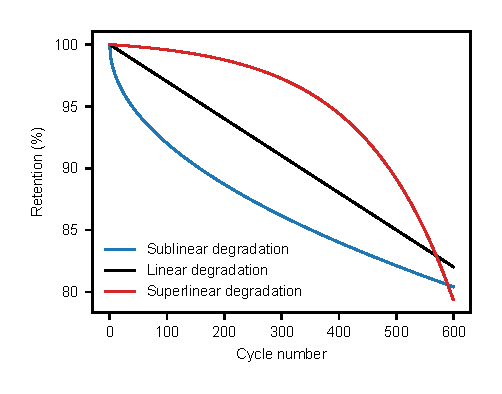
\includegraphics[scale=1]{figures/degradation_rates.eps}
\caption{Schematic of the three lithium-ion battery aging trajectories observed in the literature: sublinear, linear, and superlinear degradation (``knees''). Knees pose challenges for long battery lifetimes. Here, the $x$ axis is labeled ``cycle number'', although it could also represent equivalent cycles or similar; similarly, the $y$ axis is labeled ``retention'', although it could also represent absolute capacity, energy, or power. We use this convention (``retention vs. cycle number'') in conceptual figures throughout this work.}
\label{fig:degradation_shapes}
\end{figure}


In this review, we survey the literature and critically examine both experimental and modeling work on the subject of knees in lithium-ion battery aging. We first review methods to identify the knee point from an aging trajectory. We then identify six knee ``pathways'' from the literature, including lithium plating, cathode saturation, resistance growth, additive depletion, percolation-limited connectivity, and mechanical deformation. We also classify differences in experimentally observed knee behavior as either differences in design, differences in usage conditions, or cell-to-cell/testing variation. Finally, we discuss the implications of our review to both predicting and avoiding knees, and we suggest future work on this topic. This review can serve both academic and industrial efforts to understand and improve lithium-ion battery lifetime.

\section{Defining the knee point}

% \pbox{
% Key messages in my mind:
% \begin{itemize}
%     \item Knees seem easy to identify by eye, and have a nice mathematical description as the second derivative \cmark 
%     \item However noise makes this nontrivial (figure) \cmark
%     \item No formal definition (IEEE standard) \cmark
%     \item Briefly describe different methods
%         \subitem SG: We don't want this to take up too much space. If possible, a single plot with diagrams should suffice. \cmark
% \end{itemize}
% }

Mathematically, the knee is described as the point at which the degradation rate is changing fastest, i.e., the second derivative reaches some maximal value. In regard to batteries, IEEE Standard 485\texttrademark-2010  \cite{noauthor_ieee_2011} defines a (capacity) knee as a change to a stage of rapid decrease in capacity. However, this definition is qualitative and thus hard to apply in practice: while the \textit{presence} of a knee is generally straightforward to identify, the \textit{location} of a knee is less so. 
Locating a knee by eye is a seemingly plain task for a single, smooth and ideal aging profile (e.g.,~the superlinear aging trend in Figure \ref{fig:degradation_shapes}). Nonetheless, Figure \ref{fig:knee_definition3} demonstrates the problem of using a second derivative to identify the knee point with small amounts of noise (standard deviation of 0.05\% capacity, green) or with limited data points (blue) where the knee is artificially shifted later. The data is too discrete in either of these limiting cases. Furthermore, in deployed systems, varying duty cycles can effectively manifest as ``noise'' in estimates of capacity or energy.
Consequently, \cite{strange_elbows_2021} concluded that health metric profiles should be smoothed prior to knee identification, but aging trajectories with few data points need more attention.

\begin{figure}[ht]
\centering
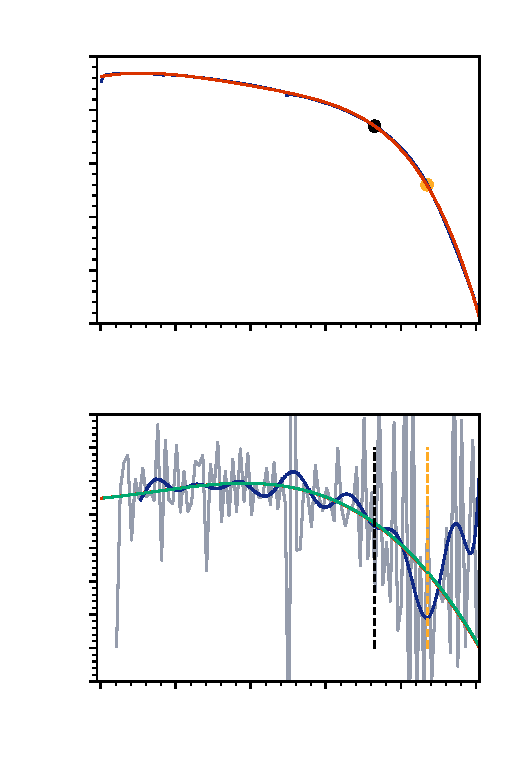
\includegraphics[scale=1]{figures/knee_definition.eps}
\caption{(a) Defining the knee point. The position of knee point as visually identified by an author (black point) differs from the mathematically defined knee point (yellow point). Data from batch 2, channel 12 cell from Severson et al.\cite{severson_data-driven_2019} The capacity is normalized by the nominal capacity of the cell. (b) Vulnerability of knee detection methods to noise.}
\label{fig:knee_definition3}
\end{figure}



\begin{figure}[h!tb]
\centering
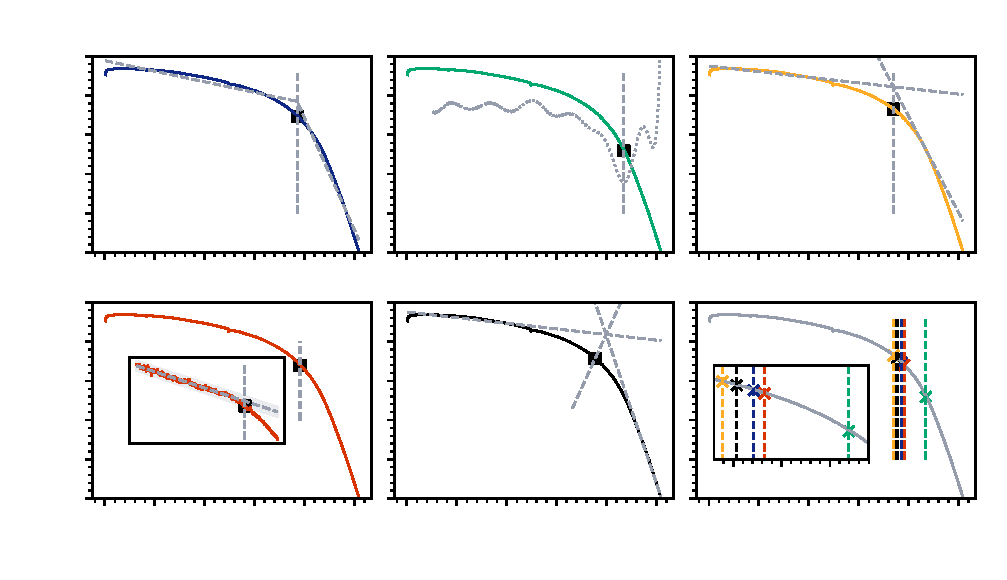
\includegraphics[scale=1]{figures/knee_identification_methods.eps}
\caption{Different knee identification methods exemplified on the cell from batch 2, channel 12 of Severson et al.\cite{severson_data-driven_2019}. The capacity is normalized by the nominal capacity of the cell. (a) Bacon-Watts \cite{fermin-cueto_identification_2020}, (b) Kneedle \cite{satopaa_finding_2011} (where the second derivative is also shown as a dotted gray line), (c) tangent-ratio from Diao et al.\cite{diao_algorithm_2019}, (d) Zhang et al.\cite{zhang_identifying_2020}, (e) Bisector from Greenbank and Howey(cite eventually). (f) Comparison of knee points as identified via these methods. 
(
WAIT UNTIL END TO ADD CITATIONS IN THE TEXT )}
\label{fig:knee_identification_methods}
\end{figure}

Several ``offline'' knee point identification methods have been proposed in the literature.
``Kneedle'' calculates the knee as the point of maximum curvature of the capacity curve \cite{satopaa_finding_2011}. The knee has also been calculated using the ``Bacon-Watts'' method for estimating the transition between two intersecting lines fitted to a capacity fade curve, a method which can also provide an estimate of the ``knee-onset'', the point where the aging trajectory is no longer linear \cite{fermin-cueto_identification_2020}. Other methods use tangential lines, such as the ``tangent-ratio'' (which defines the knee based on a tangent ratio at the inflection and maximum slope points of the capacity curve)\cite{diao_algorithm_2019} and the bisector method (which uses linear extrapolations of early and late life then an angle bisector identifies the knee as it intersects the capacity curve)\textbf{CITE-SAM\&David}. Finally, Zhang et al.\cite{zhang_accelerated_2019} proposed approximating early life with a linear regression, then defining a cell to have a knee if the capacity fell below a defined band about that regression line. The region is calculated using the variation in the height of a voltage peak; other methods do not require the use of voltage data (working only with the capacity curve). Of these five methods, the Bacon Watts and bisector methods are (arguably) the easiest to implement since they both avoid the use of derivatives and voltage data.

In Figure \ref{fig:knee_identification_methods}, we implemented and applied these methods to a single cell from Severson et al.\cite{severson_data-driven_2019}. All methods estimate the knee point at cycle numbers within a 20 cycle range (370--390 cycles) except the ``Kneedle'' method (435 cycles). These results held across most cells in the Severson et al.\cite{severson_data-driven_2019} dataset, suggesting that these methods are generally comparable for offline knee point estimation. Among these methods and testing with this dataset, the only consistent relationship found was that  ``Kneedle'' always estimates a slightly larger knee point (by 35 cycles on average) than ``Bacon-Watts''; no such relation holds for the remaining methods (see Supplementary Discussion 1 for details). 

Finding the knee online, i.e., during use, is difficult because the end-of-life capacity profile is not known and because the discharging conditions are inconsistent. Transforming the offline methods into online methods is challenging since many of these methods require the entire aging trajectory for knee point estimation. However, the method of Zhang et al.\cite{zhang_accelerated_2019} can accommodate online knee point estimation since only the initial aging trajectory is required. Of course, the challenge of uncontrolled usage conditions is inherent to online state estimation; varying duty cycles in deployed systems could mask the knee.



%%%%%%%%%%%%%%%%%%%%%%%%%%%%%%%%%%%%%%%%%%%%%%%%%%%%
%%%%%%%%%%%%%%%%%%%%%%%%%%%%%%%%%%%%%%%%%%%%%%%%%%%%
%%%%%%%%%%%%%%%%%%%%%%%%%%%%%%%%%%%%%%%%%%%%%%%%%%%%
%%%%%%%%%%%%%%%%%%%%%%%%%%%%%%%%%%%%%%%%%%%%%%%%%%%%


\section{Pathways for knee points}

We surveyed the literature and identified six ``knee pathways''. These pathways are schematically illustrated in Figure \ref{fig:knee_pathways}. Some of these pathways (e.g., lithium plating) have been extensively characterized and modeled, while others (e.g., percolation-limited knees) are merely hypotheses. Here, we critically examine the evidence for each pathway. For more extensively studied pathways such as lithium plating, we consider both \textit{modes}, defined as high-level changes in cell state, and \textit{mechanisms}, defined as the specific failure that leads to a change in cell state. For instance, active material loss is a degradation mode that can be caused by electrode delamination, one of several possible failure mechanisms for this degradation mode. Failure mechanisms are often challenging or impossible to pinpoint exactly or experimentally isolate, but failure modes are usually identifiable through common electrochemical measurements or characterization methods and can be considered to conceptually validate a proposed pathway.

\begin{figure}[h!tb]
\centering
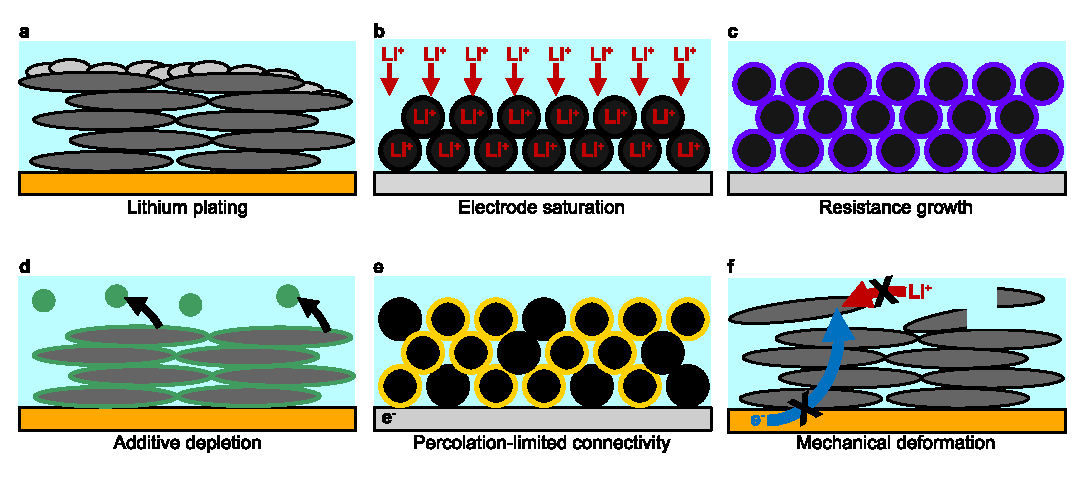
\includegraphics[scale=1]{figures/knee_pathways.eps}
\caption{Schematics of the six ``knee pathways'' identified in the literature. Each of these pathways may have multiple degradation modes (e.g., loss of active material), and each of these modes may have multiple degradation mechanisms (e.g., electrode delamination). This figure emphasizes particle- and electrode-level effects, although many of these mechanisms occur on the nano- and macroscales as well.
(a) Lithium plating, in which metallic lithium deposits on the surface of the negative electrode particles.
(b) Electrode saturation, in which the number of active sites in the electrode constrains the lithium inventory.
(c) Resistance growth, in which high overpotentials leads to a rapid drop in available capacity.
(d) Additive depletion, in which the depletion of a critical additive triggers a knee.
(e) Percolation-limited connectivity, in which a small change in ionic or electronic electrode connectivity leads to a large change in electrode active material.
(f) Mechanical deformation, in which microscale, mesoscale, or macroscale mechanical effects trigger an increasing rate of active material loss.}
\label{fig:knee_pathways}
\end{figure}

We also consider the relationship between the observable state variables (i.e., capacity, energy, and power) and the mechanisms underlying their knee points. Figure \ref{fig:snowball_vs_hidden_vs_threshold} illustrates three underlying mechanisms that can lead to a knee. \textit{Snowball} mechanisms (Figure \ref{fig:snowball_vs_hidden_vs_threshold}a and \ref{fig:snowball_vs_hidden_vs_threshold}d) occur when the underlying state variable has a direct relationship with the observable state variable, but the underlying state variable is exponentially increasing. \textit{Hidden} mechanisms (Figure \ref{fig:snowball_vs_hidden_vs_threshold}b and \ref{fig:snowball_vs_hidden_vs_threshold}e) occur when the observable state variable, originally controlled by a slowly-increasing state variable, becomes dominated by a second rapidly-increasing state variable. Finally, \textit{threshold} mechanisms (Figure \ref{fig:snowball_vs_hidden_vs_threshold}c and \ref{fig:snowball_vs_hidden_vs_threshold}f) occur when the observable state variable changes when the underlying state variable reaches a threshold. Each of these underlying mechanisms has unique implications for detectability and prediction, a point we return to throughout this work.

\begin{figure}[h]
    \centering
    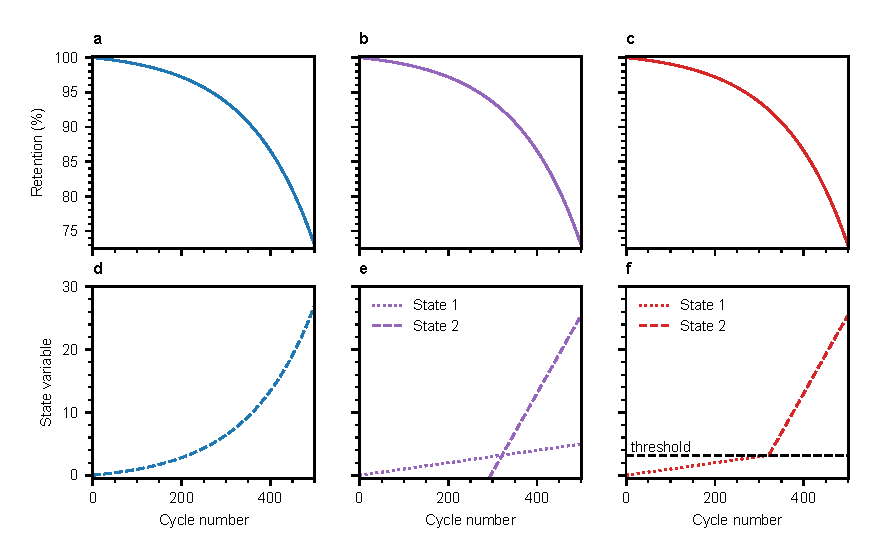
\includegraphics[scale=1]{figures/snowball_vs_hidden_mechanism.eps}
    \caption{Schematic of the three types of underlying mechanisms leading to a knee. In each case, the retention curve looks the same (a-c), but the underlying mechanism has a different functional form. (d) ``Snowball'' mechanism, in which the state variable is exponentially increasing. (e) ``Hidden'' mechanism, in which a slowly-increasing state variable is dominated by a rapidly-increasing state variable. (f) ``Threshold'' mechanism, in which a dramatic change in observable state is triggered by a state variable reaching a threshold.}
    \label{fig:snowball_vs_hidden_vs_threshold}
\end{figure}

\subsection{Lithium plating knees}

\pbox{
I still need to make a figure for all Li plating modes
}

Lithium plating occurs when lithium ions form metallic lithium on the surface of the electrode rather than intercalating into it. The plating reaction is favorable when the reaction potential of Li/Li$^+$ is greater than the equilibrium potential for other alternative reaction pathways for Li$^+$ (i.e., graphite intercalation).\cite{gao_interplay_2021} Plating can occur due to either ``thermodynamic plating'', or plating that occurs independent of the applied current, and ``kinetic plating'', or plating that only occurs if the applied current exceeds some value.  Furthermore, lithium plating can occur either reversibly or irreversibly. Irreversible plating leads to rapid loss of lithium inventory and has historically been considered to be a primary driver for capacity knees. We generally refer to irreversible plating throughout this discussion.

Generally, lithium plating on graphite follows heterogeneous nucleation and growth kinetics, in which rapid growth proceeds quickly after an initial nucleation phase.\cite{ely_heterogeneous_2013, pei_nanoscale_2017, gao_interplay_2021}
Thus, lithium plating can often be considered a ``snowballing'' knee (Figure \ref{fig:snowball_vs_hidden_vs_threshold}a and \ref{fig:snowball_vs_hidden_vs_threshold}d). However, some lithium plating pathways (e.g., lithium plating driven by active material loss from the negative electrode) will exhibit knees independent of the nucleation and growth of plated lithium.

Here, we discuss the mechanisms by which plating can lead to a knee (Figure X). We suggest Waldmann et al.\cite{waldmann_li_2018} and Gao et al.\cite{gao_interplay_2021} for comprehensive general overviews of lithium plating.

% Intro to plating
% \begin{itemize}
%     \item What is Li Plating?
%     \item Why does plating occur generally (V<Li)
%     equilibrium potential of the Li$\mathrm{^0}$/Li$\mathrm{^+}$ > everything else
%     \item Brief introduction to and definition of each plating pathway
%     \subitem Thermodynamic "non-current-induced"
%     \subitem Kinetic "current induced"
% \end{itemize}

\subsubsection{Thermodynamic lithium plating}

%- x$>0$
%- heterogeneous temperature
%- ${LAM}_{de}$NE

Thermodynamic lithium plating occurs whenever the lithium capacity during charging exceeds the negative electrode capacity, i.e., the negative electrode is unable to host all of the lithium from the positive electrode. Generally, the latter can be avoided in fresh cells by simply using a negative electrode to positive electrode capacity ratio (n:p ratio) greater than 1. However, if active material from the negative electrode is lost during aging, thermodynamic lithium plating will occur even in cells with excess negative electrode capacity.

\paragraph{Thermodynamic lithium plating in fresh cells}

While thermodynamic lithium plating in fresh cells can be easily avoided by proper cell design, this degradation mechanism is often exploited for scientific studies of lithium plating.
For instance, Deichmann et al.\cite{deichmann_investigating_2020} created cells with n:p ratios of 0.75 and 0.5 to intentionally deposit lithium metal on graphite electrodes. The authors identified a relationship between decreased n:p and capacity fade, which they attributed to high loss of lithium inventory using differential capacity analysis and SEM. In a creative study, Martin et al.\cite{martin_cycling_2020} used deposited lithium metal as a mechanism to store extra capacity, enabling the cell to occasionally discharge extra energy (i.e., when extra range is needed) without requiring a substantially larger negative electrode. This cell design used an n:p ratio of 0.6, where n:p is calculated using the lithium capacity of the conventional graphite. A high upper cutoff voltage during charging was used to intentionally plate lithium onto graphite; unsurprisingly, irreversible lithium plating was found to be the primary failure mechanism, with over 50\% capacity loss of lithium metal in two of the three electrolytes tested.

\paragraph{Thermodynamic lithium plating due to loss of active material}

Loss of active material --- specifically, loss of active material from the delithiated negative electrode ($\mathrm{LAM_{deNE}}$) --- during aging may result in thermodynamic lithium plating if the lithium capacity of the negative electrode becomes the limiting factor during charging. For instance, if the rate of $\mathrm{LAM_{deNE}}$ exceeds that of the loss of lithium inventory (LLI), the negative electrode will eventually be unable to accommodate all lithium during charging, which will lead to thermodynamic lithium plating and thus a knee. Dubarry et al.\cite{ansean_operando_2017, dubarry_durability_2018, baure_synthetic_2019, dubarry_big_2020} have extensively explored this scenario in multiple studies, considering different ratios of $\mathrm{LAM_{deNE}}$ to LLI as well as different extents of reversible and irreversible plating (Figure \ref{fig:thermo_plating}). This case is a prototypical case of a hidden state (i.e., loss of active negative electrode material) causing a knee.

\begin{figure}[p]
    \centering
    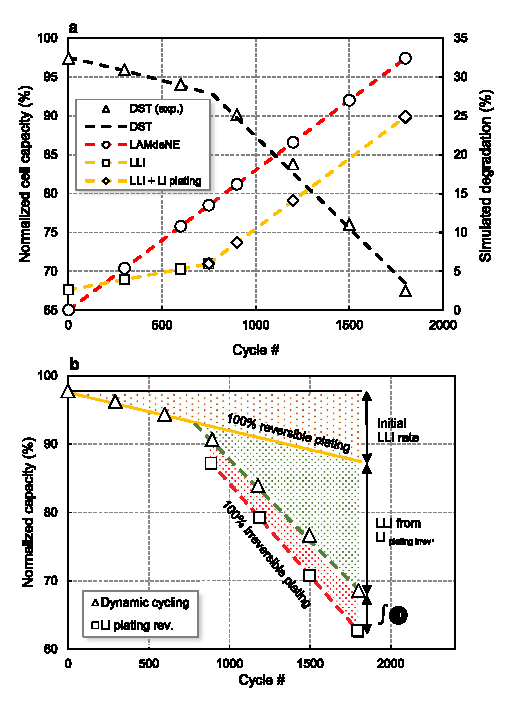
\includegraphics[scale=1]{figures/thermo_plating_dubarry.eps}
    \caption{Thermodynamic lithium plating driven by loss of active negative electrode material. (a) Evolution of aging parameters with cycling of cell degradation. The left axis shows the experimental normalized cell capacity (triangle markers), and the dashed black line shows the results of cell capacity simulations with the calculated aging modes. The right axis shows the evolution of the degradation induced by the calculated aging modes (markers and dashed lines) with cycling. Note that $\mathrm{LAM_{deNE}}$ increases linearly, and at a rate higher than LLI.
    (b) Capacity vs. cycle number at low rate (C/25), depicting the contributions to the total capacity fade as a function of cycle number.
    Adapted from Figures 7 and 8 of Anse\'an et al.\cite{ansean_operando_2017}}
    \label{fig:thermo_plating}
\end{figure}

Various degradation mechanisms can lead to $\mathrm{LAM_{deNE}}$, which occurs when active sites lose either ionic or electronic connectivity with the electrode.
Often, several of these mechanisms can occur in parallel, leading to a snowball effect where loss of active material due to one mechanism may result in further stress on the remaining active sites, accelerating degradation via thermodynamic lithium plating.
Electrode sites can lose electronic connection via delamination\cite{liu_aging_2010, cannarella_stress_2014, somerville_effect_2016, willenberg_high-precision_2020}, particularly for cells with low external pressure\cite{cannarella_stress_2014}. Particle cracking is another mechanism for electronic disconnection of active sites, although cracking is not expected to occur appreciably in graphite particles.\cite{takahashi_examination_2015}
Electrode sites can lose ionic connection via electrolyte dry-out, which may be driven by gas generation during cycling.\cite{mao_calendar_2017, kupper_end--life_2018}
Another mechanism causing loss of active material via ionic disconnection is the growth of microns-thick ``covering layers'', a mechanism which we mention now but explore in depth in our discussion on mechanical knees.

\subsubsection{Kinetic lithium plating}
%- this is when transient effects cause plating
%- Low T -> Low D -> High Surface x -> ${eta}_{s}$<0
%- Low OCV + High ${eta}_{op}$ -> ${eta}_{n}$<Li
%- High σ -> Low ρ -> High Surface x -> ${eta}_{s}$<0
%- SEI -> Low ρ -> High Surface x ->${eta}_{s}$<0

``Kinetic'' lithium plating occurs when excessive transport or reaction overpotentials cause the local electrode potential to drop below that of Li/Li$\mathrm{^+}$.
In other words, kinetic lithium plating occurs at conditions when the plating could otherwise be mitigated by lithiating the graphite at a sufficiently low current. As Gao et al.\cite{gao_interplay_2021} describe, salt depletion in the electrolyte, poor charge transfer kinetics, and surface crowding in the graphite at the graphite surface further favor lithium plating over intercalation. While kinetic lithium plating can occur via similar mechanisms to thermodynamic lithium plating, the dynamic nature of this process introduces additional avenues for lithium plating knees to occur.

\paragraph{Kinetic lithium plating in fresh cells}
Kinetic lithium plating can be driven by a wide range of cell designs and usage conditions; the prototypical use case leading to lithium plating is high charging rates at low temperature \cite{waldmann_temperature_2014, petzl_lithium_2015}. Waldmann et al.\cite{waldmann_temperature_2014} observed an increase in the rate of aging with a decrease in temperature below 25$^{\circ}$C, attributing the increased aging rate to lithium plating via dissections. Low temperatures increase both the transport overpotentials for lithium ions within the electrolyte and electrode and the reaction overpotential for litihum intercalation. Note that ``high'' charging rate or ``low'' temperature do not have consistent quantitative definitions, as plating will occur whenever the local potential exceeds the energy barrier for lithium nucleation. Thus, plating may be observed even at ``standard'' test conditions, such as 1C constant-current charging near room temperature \cite{waldmann_optimization_2015,burns_-situ_2015}. Increasing temperature and improved cell design (i.e., thinner electrodes) may allow for much more rapid charging before lithium plating and knees are observed; Lewerenz et al.\cite{lewerenz_systematic_2017} cycled cells at rates up to 8C, observing no knees at rates as high as 4C, though microstructural evidence of plating was found even at 1C. The onset of lithium plating is also sensitive to the charging protocol, with many studies demonstrating that informed design of charging protocols can substantially extend cell lifetime by preventing direct lithium plating.\cite{waldmann_optimization_2015,schindler_fast_2018}. Optimizing electrode architectures to improve electrolyte transport kinetics is a further path forward to increase charging currents without lithium plating.\cite{nemani_design_2015, usseglio-viretta_enabling_2020}

Mechanical stress may also lead to kinetic lithium plating, as applied stress can compress the electrode or separator. This compression locally decreases the porosity of the electrodes, reducing the diffusivity of electrolyte and thus increasing the local polarization and causing lithium plating. Cannarella and Arnold\cite{cannarella_stress_2014} conducted a direct test of this mechanism, finding that high external pressures can induce lithium plating in pouch cells and directly leading to a knee. In a follow-up experiment, Liu and Arnold\cite{liu_effects_2020} demonstrated that localized lithium plating could be induced in densified regions of the separator. 

\paragraph{Kinetic lithium plating due to loss of active material}
As previously discussed, a hidden mechanism for thermodynamic lithium plating is loss of delithiated negative electrode active material.\cite{ansean_operando_2017, dubarry_durability_2018, baure_synthetic_2019, dubarry_big_2020} Mechanisms for loss of active material include delamination, particle cracking, electrolyte dry-out, and covering layer growth. However, $\mathrm{LAM_{deNE}}$ can also drive kinetic lithium plating, even if the negative electrode capacity does not limit the charging capacity. Active material loss without a corresponding loss in lithium flux will lead to an increased local current density on the negative electrode surface; these high local current densities can drive lithium plating.

Continuous active material loss will create increasingly larger local current densities, which will drive increasingly larger lithium plating potentials. Thus, in kinetic plating regimes, linearly increasing active material loss can cause accelerating rates of lithium plating. Furthermore, as previously discussed, the nucleation and growth kinetics of lithium plating also serves as a snowball mechanism, since growth of nucleated phases can occur rapidly. This ``double-snowball'' effect is especially pernicious and is expected to lead to sharp knees. To our knowledge, prior experimental or modeling work has not considered this effect. Overall, this effect highlights the risks from negative electrode active material loss.

\paragraph{Kinetic lithium plating due to pore clogging}
As SEI grows, it precipitates mainly in the pores of the anode, decreasing the available volume fraction for electrolyte in the electrode \cite{sikha_effect_2004}. The decreased volume fraction increases the electrolyte transport overpotentials, which can ultimately lead to lithium plating. The plated lithium, which has a much lower density than intercalated lithium\cite{yang_modeling_2017}, further decreases the porous volume fraction, creating a positive feedback loop for additional lithium plating\cite{yang_modeling_2017}. Modeling studies of this phenomenon have observed that a critical porosity exists around 0.05, beyond which a knee occurs \cite{yang_modeling_2017, muller_model-based_2019}. This effect has also been modeled by simply decreasing the diffusion coefficient as a function of cycle number \cite{keil_electrochemical_2020}. One proposed countermeasure for this issue is to use a graded or stepped porosity profile through the thickness of the negative electrode. Since most pore clogging occurs near the separator, having a higher porosity near the separator and a lower porosity near the current collector can slow the onset of the knee caused by pore clogging \cite{muller_model-based_2019}.
While this mechanism has not been experimentally validated, decreasing anode porosity with cycling has been observed via X-ray computed tomography of samples of a graphite electrode.\cite{frisco_understanding_2016, rahe_nanoscale_2019} Furthermore, the ``covering layer'' effect discussed at a later point may be related to this phenomenon, as models of plating induced by pore clogging suggest that the pore clogging occurs primarily at the separator-electrode interface.\cite{yang_modeling_2017}

\begin{figure}
    \centering
    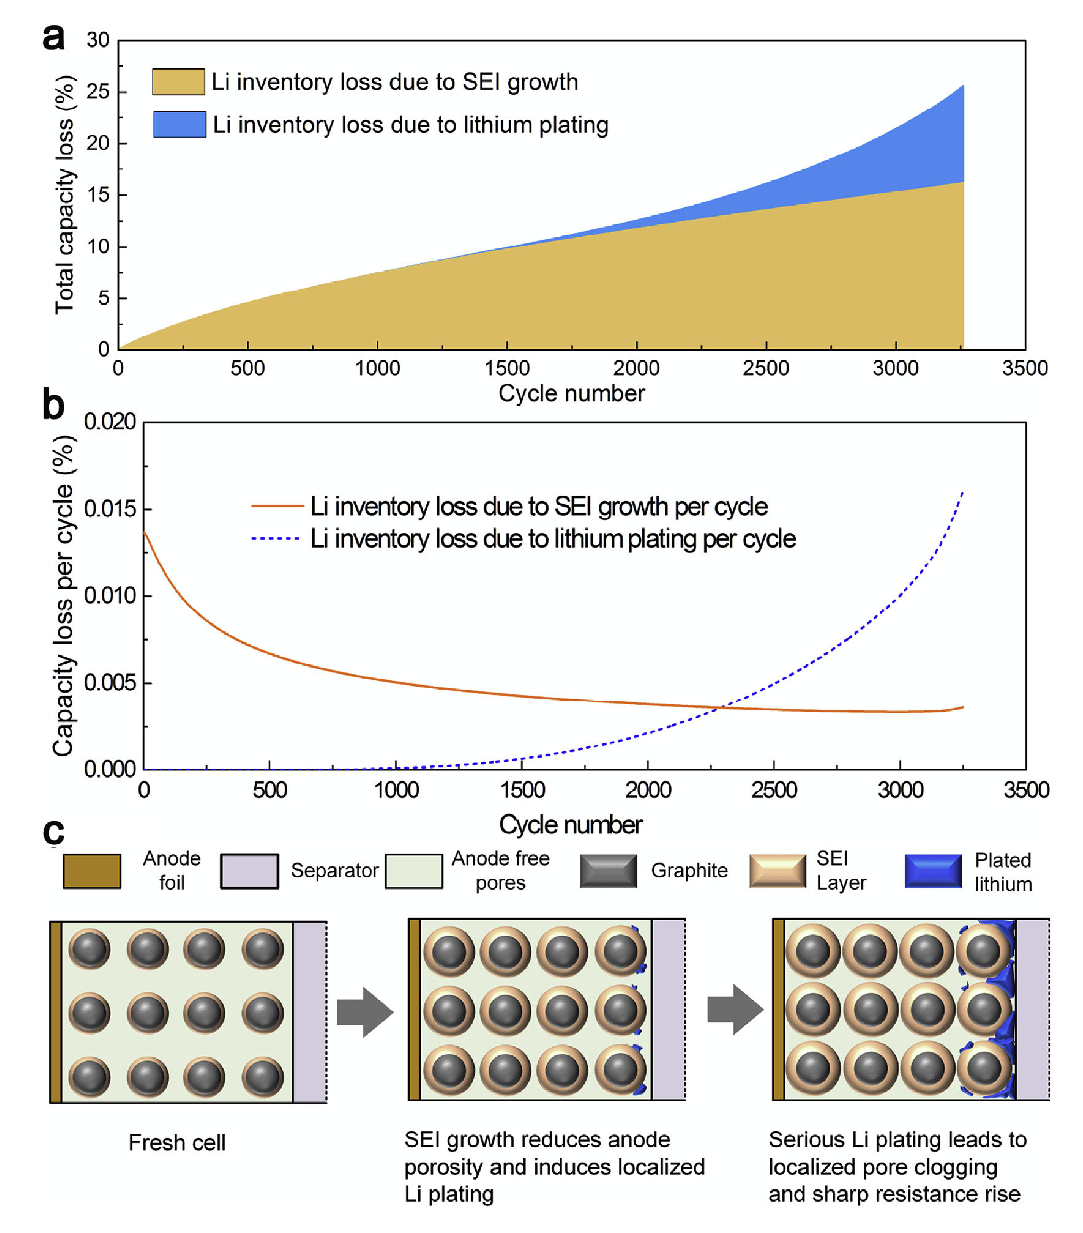
\includegraphics[scale=0.7]{figures/li_plating_porosity_yang.eps}
    \caption{Kinetic lithium plating due to pore clogging. (a) Lithium inventory loss contributed by SEI growth and lithium plating, respectively. (b) Lithium inventory loss per cycle contributed by SEI growth and lithium plating, respectively. The ``snowballing'' growth of lithium plating occurs due to the accelerating decrease in porosity, which creates high transport overpotentials in the electrolyte and drives additional plating. (c) Schematic illustration of pore clogging driven initially by SEI growth and then by plating. Adapted from Figure 8 of Yang et al.\cite{yang_modeling_2017}}
    \label{fig:pore_clogging}
\end{figure}

\subsection{Electrode saturation}

\pbox{Need to add new figure, Tino's figure, text around Tino's figure}

As previously discussed, lithium plating can occur if the active sites in the negative electrode cannot accommodate the available lithium inventory. More generally, if the rate of active material loss for one electrode outpaces the rate of lithium inventory loss, the electrode can ``saturate'' and reach the cutoff potential well before all lithium has transferred. If this electrode is not limiting, its loss of active material will be hidden from the overall capacity until this electrode becomes limiting; furthermore, if the rate of active material loss is sharper than the initial rate of lithium inventory loss, a knee in capacity will manifest. Dubarry et al.\cite{dubarry_synthesize_2012} and Smith et al.\cite{smith_life_2017} captured this knee pathway by using a more aggressive functional form for active material loss than lithium inventory loss (Figure X). This mechanism can apply for either electrode, but loss of active material from the negative electrode is more likely to be a hidden mechanism since this electrode is typically oversized relative to the positive electrode; the exception is cells with lithium titanate electrodes, in which the positive electrode is limiting and can cause a ``hidden'' knee(cite baure-battery-2019, baure-battery-2020).

\begin{figure}
\centering
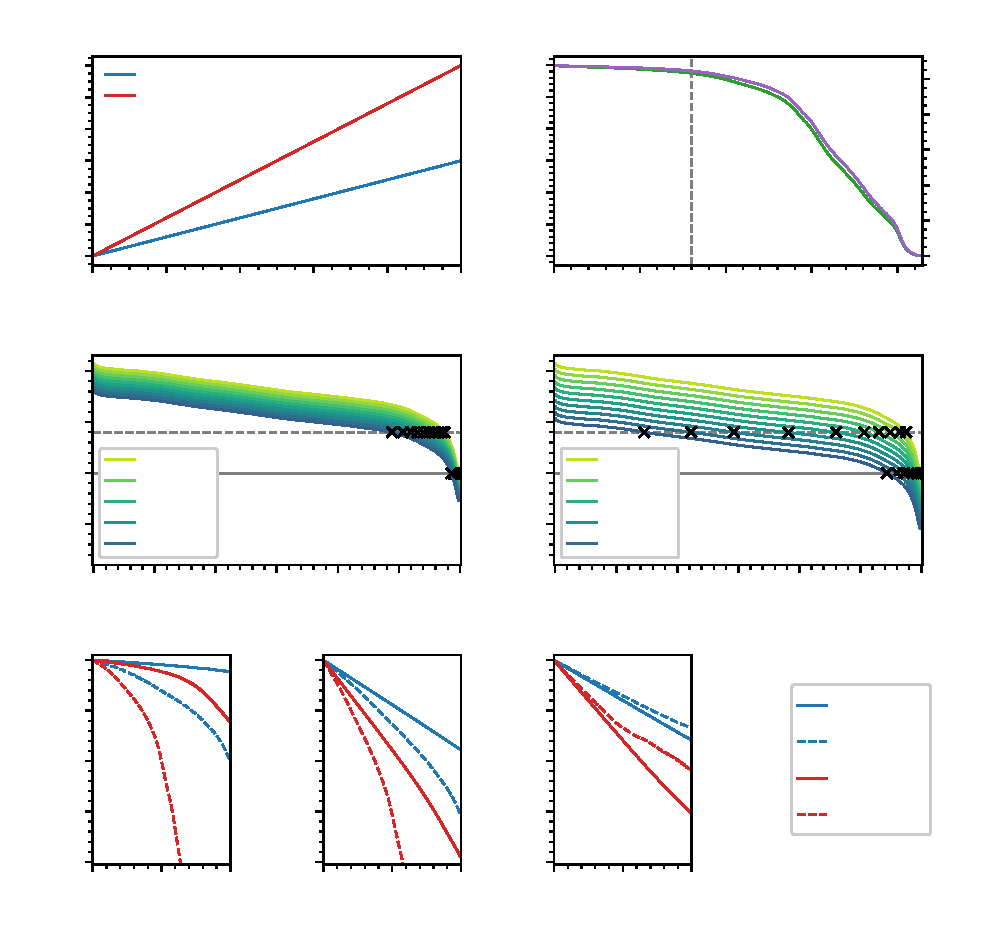
\includegraphics[scale = 1]{figures/dcr_growth_knee_2.eps}
\caption{Simple model illustrating ``pseudo-knees'' due to resistance growth; we use the term ``pseudo-knees'' here since the knee location is a function of rate and lower cutoff voltage. Inspired by Figure 16 of Ma et al.\cite{ma_editors_2019} and Mandli et al.\cite{mandli_analysis_2019}. (a) Assumed overpotential growth vs. cycle number for a 1C and 2C discharge. The assumed resistance growth rate is 0.2 m$\Omega$/cycle. (b) Discharge capacity and energy vs. the minimum discharge voltage for an example NMC/graphite cell. Data obtained from Preger et al.\cite{preger_degradation_2020} (c, d) Voltage vs. capacity as a function of cycle number for the (c) 1C discharge and (d) 2C discharge cases. The final discharge capacity for each cycle is denoted by a marker. (e--g) (e) Capacity, (f) energy, and (g) power retention vs. cycle number as a function of discharge current and the minimum voltage.
}
\label{fig:dcr_knee}
\end{figure}

A richer picture emerges in models that capture the shifts in electrode stoiciometry with cycling. Lin et al.~\cite{lin_comprehensive_2013} modeled loss of lithium inventory driven by SEI growth and loss of active material driven by mechanical effects in the positive electrode. This loss of active material widens the positive electrode utilization window due to the increased ratio of lithium inventory to positive electrode active sites, which increases the cell voltage for a given amount of transferred lithium. This effect reduces the capacity between the voltage limits. The knee occurs when the positive electrode becomes fully saturated before the entire lithium inventory is transferred.

Sulter et al.(cite preprint) replicated a similar mechanism in Figure X...

\subsection{Resistance growth-induced knees}

Cell internal resistance often increases during aging due to the growth of side reaction products on the surface of the electrode particles, particularly on the cathode(). Under constant current conditions, the additional overpotential from increased internal resistance will cause the cell to reach the cutoff voltage more quickly, decreasing the capacity, energy, and power per cycle. The magnitude of this overpotential growth rate is a product of both the resistance growth rate (i.e., electrolyte reaction rate) and the applied current.

Most modern lithium-ion batteries have voltage-capacity curves that are relatively flat at higher voltages/SOCs (i.e., large d$V$/d$Q$) and relatively steep at lower voltages/SOCs (i.e., small d$V$/d$Q$). Thus, the charge capacity (excluding the constant-voltage portion) is highly sensitive to small increases in resistance growth. In contrast, the discharge capacity is less sensitive to resistance growth---until the overpotential is large enough such that the discharge ends in the flatter region of the voltage-capacity curve (i.e., a small increase in overpotential leads to a large decrease in capacity). When this flatter region is reached, the discharge capacity becomes more sensitive to small changes in overpotential, leading to a knee in capacity, energy, and power.

Figure \ref{fig:dcr_knee} displays a simple model illustrating knee onset due to ohmic resistance growth during cycling, inspired by the work of Ma et al.\cite{ma_editors_2019} and Mandli et al.\cite{mandli_analysis_2019}. The model assumes a constant resistance growth rate of 0.2 m$\Omega$ per cycle, occurring at all SOCs; the linearly increasing resistance with cycle number leads to linearly increasing ohmic overpotential (Figure \ref{fig:dcr_knee}a). The increased overpotential then shifts the voltage-capacity curve downwards.
To demonstrate the impact of increasing resistance due to this downshift in a ``real'' cell, we used voltage-capacity and voltage-energy relationships recorded from an NMC/graphite cell at beginning-of-life from Preger et al.\cite{preger_degradation_2020} (Figure \ref{fig:dcr_knee}b). Figures \ref{fig:dcr_knee}c and \ref{fig:dcr_knee}d show the impacts of this downshift on the voltage-capacity curve at lower voltage cutoffs of 2 V and 2.8 V and discharge currents of 1C (Figure \ref{fig:dcr_knee}c) and 2C (Figure \ref{fig:dcr_knee}d). In all cases, the discharge ends on the steep portion of the voltage-capacity curve at the beginning of life. But as the cell ages and the resistance increases, the discharge ends on the flat region of the voltage-capacity curve, resulting in an increased rate of capacity loss (i.e., a knee) despite a linear increase in resistance. Thus, this knee pathway is a threshold mechanism, where the state variable is the overpotential and the threshold is the ``overpotential margin'' between the lower cutoff voltage and the flatter region of the voltage-capacity curve.

The impact of the resistance growth on the measured capacity (Figure \ref{fig:dcr_knee}e), energy (\ref{fig:dcr_knee}f), and power (\ref{fig:dcr_knee}g) during discharge is highly sensitive to the discharge rate and the lower cutoff voltage---usage parameters that are not often considered critical for their impact on knees. Lower rates, of course, decrease the overpotential and delay the onset of the knee. Lower cutoff voltages delay the knee by increasing the overpotential margin between the lower cutoff voltage and the flatter region of the voltage-capacity curve; however, note that low cutoff voltages can also induce additional degradation mechanisms such as copper dissolution(fear-elucidating-2018, carter-xray-2018). Naturally, energy and power knees (\ref{fig:dcr_knee}f, \ref{fig:dcr_knee}g) are more sensitive to rate than the capacity knees (\ref{fig:dcr_knee}e). Because these knees can ``disappear'' by cycling at lower rates or to lower cutoff voltages, we sometimes refer to these knees as ``pseudo-knees''; furthermore, this knee mechanism may not be observed in some practical settings (e.g., the slow weeks-long discharge of an electric vehicle battery pack).
Finally, we note that ``resistance pseudo-knees'' may also occur due to a stoichiometric decrease of lithium available to cycle, as explored by Mandli et al \cite{mandli_analysis_2019}, or a stoichiometric shifting of lithium to one electrode preferentially during aging due to uneven loss of active material across both two electrodes \cite{lin_comprehensive_2013}.

\begin{figure}
\centering
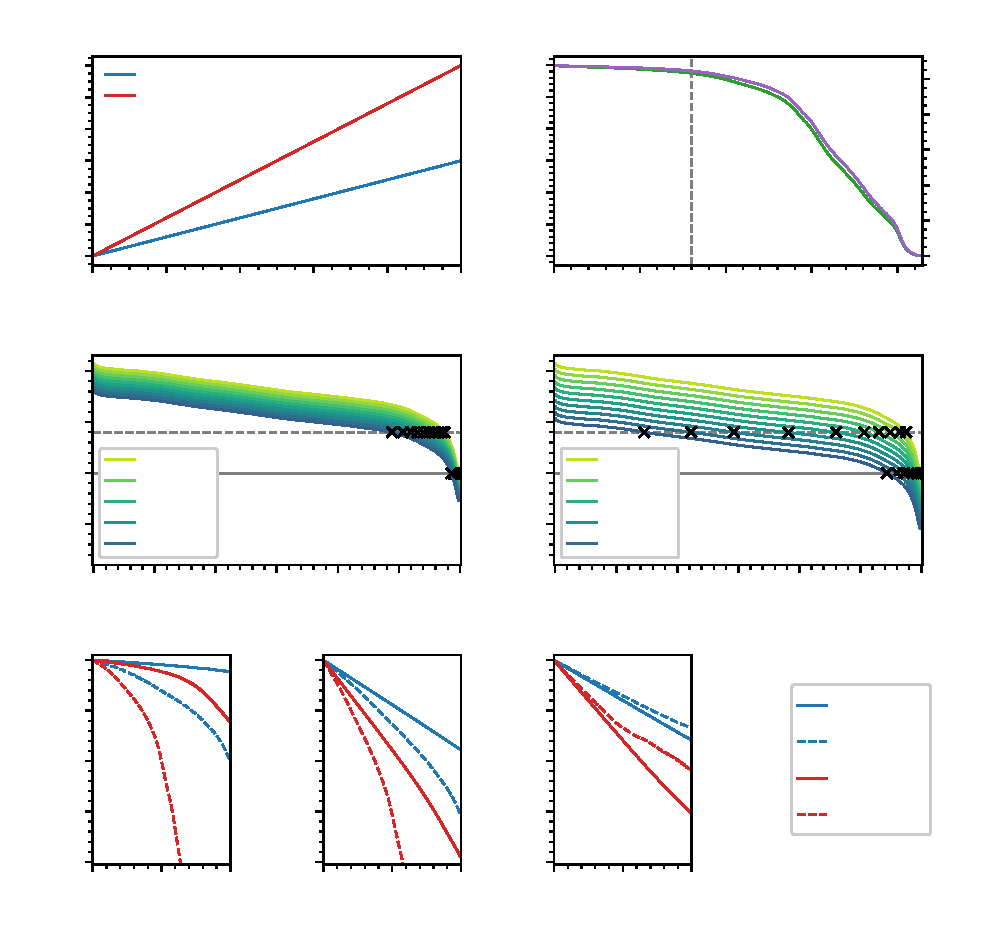
\includegraphics[scale = 1]{figures/dcr_growth_knee_2.eps}
\caption{Simple model illustrating ``pseudo-knees'' due to resistance growth; we use the term ``pseudo-knees'' here since the knee location is a function of rate and lower cutoff voltage. Inspired by Figure 16 of Ma et al.\cite{ma_editors_2019} and Mandli et al.\cite{mandli_analysis_2019}. (a) Assumed overpotential growth vs. cycle number for a 1C and 2C discharge. The assumed resistance growth rate is 0.2 m$\Omega$/cycle. (b) Discharge capacity and energy vs. the minimum discharge voltage for an example NMC/graphite cell. Data obtained from Preger et al.\cite{preger_degradation_2020} (c, d) Voltage vs. capacity as a function of cycle number for the (c) 1C discharge and (d) 2C discharge cases. The final discharge capacity for each cycle is denoted by a marker. (e--g) (e) Capacity, (f) energy, and (g) power retention vs. cycle number as a function of discharge current and the minimum voltage.
}
\label{fig:dcr_knee}
\end{figure}

Ma et al.\cite{ma_editors_2019} extensively studied this knee pathway using lab-made 230 mAh NMC532/ graphite pouch cells, varying the upper cutoff potential, discharging rate, electrolyte composition, and positive electrode material coatings. Careful impedance measurements (on both full cells and symmetric coin cells of the positive and negative electrodes) were used to identify a dramatic increase of the cathode impedance during aging. This resistance growth was attributed to electrolyte oxidation at the positive electrode, which was accelerated by high upper cutoff voltages and the use of more reactive electrodes and electrolytes (i.e., uncoated positive electrode particles, lower salt concentrations, and the use of oxidation-prone additives such as methyl acetate). One practical consideration from the work is that tests with high discharge rates exhibit resistance-growth-induced knee onsets earlier than tests with low discharge rates; thus, tests with high discharge rates can be used as an early indicator of cell knee onset at lower rates.

This knee pathway is also sensitive to electrode chemistry, as each chemistry exhibits a unique voltage-capacity curve. For instance, LFP/graphite cells experiencing high resistance growth would exhibit much sharper knees than NMC/graphite cells due to their flatter voltage-capacity curves. While LFP cells generally do not exhibit high resistance growth due to their lower operating voltages(), even moderate resistance growth coupled with high discharge rates and high lower cutoff voltages could lead to dramatic cell failure.

Lastly, we mention that capacity knees are often correlated with ``resistance elbows''---that is, a rapid rise in the resistance. While this correlation may be evidence for the prevalence of this knee pathway, other knee pathways may also lead to a resistance increase at the knee (e.g., loss of active material or porosity decrease). We return to this topic at a later point.

\subsection{Additive depletion knees}

Electrolyte additives have an disproportionate effect on lifetime relative to their presence in a cell; small quantities of electrolyte additives can often delay the occurrence of the knee by many cycles\cite{ma_editors_2019} (also cite Li 2017 comparison). Additive chemistry is complex; for instance, Burns et al.\cite{burns_predicting_2013} showed how electrolyte performance often improves with the number of additives used. Additives can influence the onset of lithium plating knees via various mechanisms (e.g., electrolyte transport properties, SEI growth rate, etc) and resistance growth knees by controlling the rate of resistance growth\cite{ma_editors_2019}. However, the \textit{depletion} of electrolyte additives is another demonstrated knee pathway. Here, we discuss perhaps the most widely studied additive depletion knee mechanism: fluoroethylene carbonate (FEC) depletion in silicon-containing cells.

FEC has been shown to substantially improve the capacity retention of silicon electrodes.\cite{choi_effect_2006, etacheri_effect_2012}
Among standard electrolyte components, FEC preferentially reacts at the surface of silicon particles; in fact, the rate of FEC consumption on silicon is 10x that of graphite, in part due to its large volume expansion (around 300\%).\cite{wetjen_differentiating_2017}
Petibon et al.\cite{petibon_studies_2016},
Jung et al.\cite{jung_consumption_2016},
and Wetjen et al.\cite{wetjen_differentiating_2017}
performed comprehensive studies of Si-containing full cells with FEC-containing electrolytes and commercially-representative volumes,
conclusively demonstrating that a knee occurs when FEC is depleted from the electrolyte.
Figure \ref{fig:fec_knee} displays key results from Petibon et al.\cite{petibon_studies_2016} and
Jung et al.\cite{jung_consumption_2016}, in which the dependence of the knee on FEC concentration was confirmed via destructive measurements of FEC concentration vs. cycle number\cite{petibon_studies_2016} and cycling cells with increasing initial FEC concentration\cite{jung_consumption_2016}.
Louli et al.\cite{louli_operando_2019} also corroborated these findings.
Earlier studies of the use of FEC in high-Si cells (cite Choi 2006, Etacheri 2012) did not observe this knee mechanism due to their use of high electrolyte volumes, which provided a large reservoir of FEC.
Other electrolyte components (namely, linear carbonates) are consumed only after the knee, since FEC can no longer be preferentially consumed\cite{petibon_studies_2016}; the cell polarization increases substantially after the knee\cite{petibon_studies_2016, jung_consumption_2016, wetjen_differentiating_2017}, possibly due to high reaction overpotential from reactions of silicon with these nonpreferred electrolyte components.
Note that this mechanism is exacerbated by high upper cutoff voltages \cite{petibon_studies_2016}, higher cycling rates (presumably due to more mechanical damage to the SEI layer) \cite{petibon_studies_2016}, and (presumably) high temperatures (due to higher SEI growth rates).

\begin{figure}[ht]
\centering
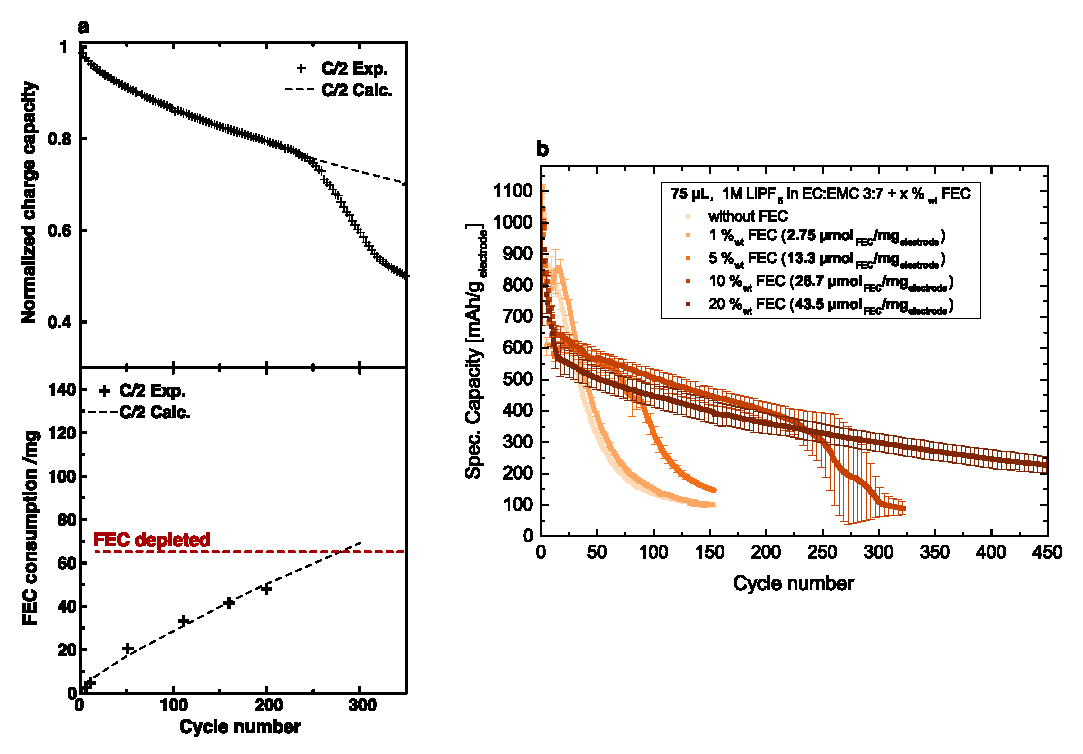
\includegraphics[scale = 0.9]{figures/fec_depletion.eps}
\caption{Additive depletion knees.
(a) The capacity retention of a full cell with 15\% Si in the negative electrode exhibits a knee at around 250 cycles, the same point at which the FEC is depleted from the electrolyte (from destructive gas chromatography-mass spectrometry measurements of FEC concentration). Adapted from Figure 8 of Petibon et al.\cite{petibon_studies_2016}
(b) In half cells with 100\% Si negative electrodes, the cycle number of the knee increases with the FEC concentration in the electrolyte. Adapted from Figure 1 of Jung et al.\cite{jung_consumption_2016}}
\label{fig:fec_knee}
\end{figure}

This knee pathway has a number of interesting implications.
First, since laboratory-built cells are often filled with high electrolyte volumes, knee mechanisms that are not present in lab testing may manifest in more commercially representative form factors.
As Wetjen et al.\cite{wetjen_differentiating_2017} emphasize,
maintaining representative electrolyte volumes in lab-scale cells is critical for accurately capturing this knee pathway in production-scale cells.
Second, nominally identical cells, cycled identically, but with different initial FEC concentrations exhibited minute electrochemical differences before the knee.\cite{jung_consumption_2016}
Theoretically, only the FEC consumed in a given cycle manifests in the electrochemical signals from cycling (e.g., differential capacity or differnetial voltage analysis); the excess FEC is not electrochemically detectable as it does not participate in reactions with the electrode.
Since the \emph{remaining} FEC amount is the main determinant of cycle life in these cells, the knee point of cells exhibiting this mechanism is not predictable via standard electrochemical signals.
An interesting proposal for future work is to evaluate other nondestructive probes (e.g., acoustic signals\cite{knehr_understanding_2018}) that may be sensitive to FEC concentration in the electrolyte.

\subsection{Percolation-limited connectivity knees}

Percolation theory \cite{essam_percolation_1980, stauffer_introduction_1994} is commonly used to describe statistical properties of clusters that are geometrically connected in porous media, including porous electrodes used in modern lithium-ion batteries\cite{ferguson_nonequilibrium_2012}. In a porous medium described by percolation theory, there exists a critical material parameter, above which the probability of a spanning cluster being formed tends towards one and below which this probability tends towards zero.\cite{ferguson_nonequilibrium_2012} In many percolating systems, this probability is highly sensitive to the value of the critical material parameter. For lithium-ion batteries, percolation theory can be used to describe both the ionic conductivity of the liquid electrolyte that fills the porous electrode and the electronic conductivity of the network of conductive additives. In battery modeling and experimentation, the electrode is often implicitly assumed to be sufficiently porous for the liquid electrolyte to completely percolate it. On the other hand, much effort has been spent on elucidating how the volume fraction of conductive additives may or may not give rise to a percolating electrically conducting network~\cite{chen_selection_2007, li_effects_2015, cerbelaud_understanding_2015, guzman_improved_2017}, which is especially important for ensuring electronic conduction is not rate-limiting in electrically insulating active materials such as lithium iron phosphate.\cite{li_effects_2015, guzman_improved_2017}

Kupper et al.\cite{kupper_end--life_2018} examined the commonly held assumption that the liquid electrolyte always percolates the porous electrode by adding a degradation mechanism that accounts for electrolyte dry-out, which results in loss of ionic contact between the active material and electrolyte and thus the subsequent loss of active material. In doing so, their model predicts ``sudden death'' of the cell capacity, which is equivalent to a knee. In this proposed electrolyte dry-out mechanism, they first define two new electrode descriptors: ``activity'', $a$, and ``saturation'', $s$, given by $a = \frac{\varepsilon_{\text{LiC}_6}}{\varepsilon_{\text{LiC}_6,\text{inactive}}+\varepsilon_{\text{LiC}_6}}$ and $s = \frac{\varepsilon_\text{elyt}}{\varepsilon_\text{elyt}+\varepsilon_\text{gas}}$, respectively. In these equations, $\varepsilon$ is the volume fraction of the active graphite ($\varepsilon_{\text{LiC}_6}$), inactive graphite ($\varepsilon_{\text{LiC}_6,\text{inactive}}$), electrolyte ($\varepsilon_{\text{elyte}}$) and gas ($\varepsilon_{\text{gas}}$, which is produced during SEI growth). The loss of ionic contact of graphite caused by electrolyte dry-out is then described by a kinetic rate law that is proportional to the difference in activity and equilibrium activity, which is assumed to be a function of only saturation. To predict a knee in cell capacity, the equilibrium activity-saturation relationships were formulated to be nonlinear and contains a percolation threshold value, around which the equilibrium activity varies rapidly between $0$ and $1$. Figure~\ref{fig:percolation} plots two such nonlinear relationships, named relationships $3$ and $4$, adapted from Figure 5 of Kupper et al.\cite{kupper_end--life_2018} which concluded that relationship 4 best fitted experimental aging data.

The knee caused by this electrolyte dry-out model is a threshold mechanism (Figure~\ref{fig:snowball_vs_hidden_vs_threshold}c \& Figure~\ref{fig:snowball_vs_hidden_vs_threshold}f), where the threshold is the critical saturation value illustrated in Figure~\ref{fig:percolation}. Although Kupper et al.\cite{kupper_end--life_2018} did not provide convincing experimental validation to definitively prove that electrolyte dry-out resulted in sudden death of the cell and that relationship 4 was the most plausible activity-saturation relationship, the proposed electrolyte dry-out mechanism is plausible in principle and should be experimentally studied in more detail. Furthermore, a similar effect may apply for electronic conductivity networks; Guzmán et al. \cite{guzman_improved_2017} illustrated how the electronic conductivity of lithium iron phosphate electrodes exhibits a percolation threshold based on the conductive carbon content.

\begin{figure}[ht]
    \centering
    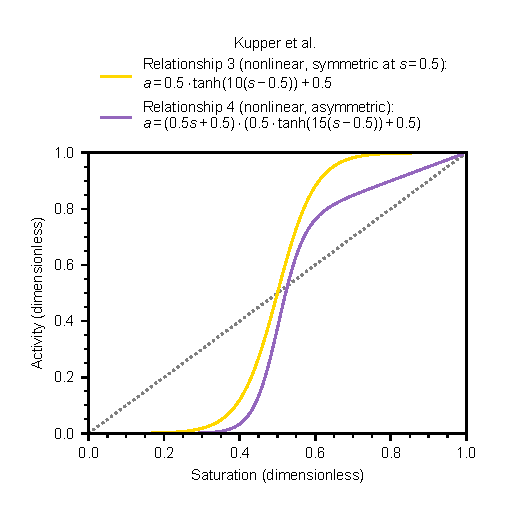
\includegraphics[scale=1.0]{figures/percolation.eps}
    \caption{Activity-saturation relationships describing percolation-limited electrolyte dry-out adapted from Figure 5 of Kupper et al.\cite{kupper_end--life_2018} Relationships 3 and 4 model percolation of the liquid electrolyte where activity depends nonlinearly on saturation. The key feature of both relationships is the presence of a percolation threshold value ($s=0.5$), around which activity varies rapidly between $0$ and $1$.
    The sensitivity of activity to small changes in saturation is apparent.}
    \label{fig:percolation}
\end{figure}

\subsection{Mechanical degradation knees}

Both microscale mechanical effects occurring at the particle scale and macroscale mechanical effects occurring at the cell scale can be pathways for knees.
Mechanical degradation mechanisms are closely tied to other knee pathways. For instance, Cannarella and Arnold~\cite{cannarella_stress_2014} showed how high external stack pressure can cause a lithium plating knee; Bach et al.\cite{bach_nonlinear_2016} demonstrated a link between heterogeneous pressure and localized lithium plating; and many loss of active material mechanisms are mechanical in nature (e.g., delamination, particle cracking, etc).
Additionally, the growth of covering layers on the anode surface, often reported on cells with knees (Figure \ref{fig:covering_layers}), \cite{lewerenz_post-mortem_2017,willenberg_development_2020,stiaszny_electrochemical_2014} may lead to additional mechanical stresses on the macroscale.
Here, we focus on knees more explicitly linked to mechanical effects.

\begin{figure}
\centering
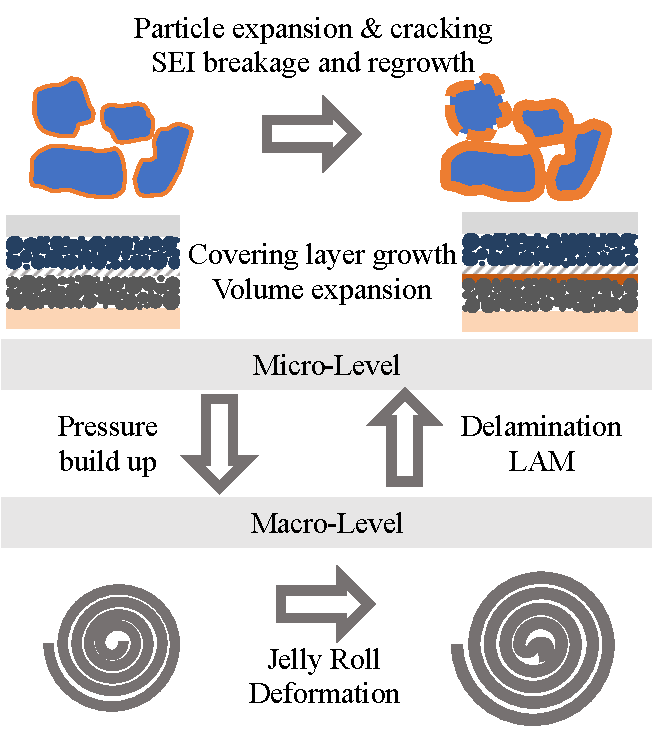
\includegraphics[scale = 1]{figures/MechanicalKneepoints.pdf}
\caption{Mechanical effects leading to knees: During cycling, particles and the SEI expand and crack, leading to the regrowth of additional SEI. In addition, covering layers may form on the surface of the negative electrode. Pressure due to volume expansion can subsequently lead to jellyroll deformation in cylindrical cells. This deformation can cause loss of active material, leading to more SEI, covering layer growth, and potentially lithium plating.}
\label{fig:knee_mechanical}
\end{figure}

At the microscale, repeated (de)intercalation can stress the electrode particles, which can then lead to both loss of active material through particle cracking and accelerated growth of side reaction products (e.g., SEI and CEI).
Reniers et al. \cite{reniers_review_2019} illustrated a positive feedback mechanism between the mechanical stress and loss of active material, leading to a (snowballing) knee point. They combine a fatigue model for loss of active material due to stress from Laresgoiti et al. \cite{laresgoiti_modeling_2015} with a stress model from Dai et al. \cite{dai_simulation_2014}: higher stress causes higher loss of active material, which in turn increases the current density and hence causes higher stress.
Other authors have suggested that mechanical effects can accelerate SEI/CEI growth by causing SEI/CEI cracking and revealing new active surface area to grow \cite{pinson_theory_2013,kupper_end--life_2018,louli_operando_2019}. Since growth of these interphasial layers is self-limiting, this effect alone is not enough to lead to a knee, but it could accelerate the onset of knees in other mechanisms related to side reactions (i.e., lithium plating induced by pore clogging on the negative electrode or resistance growth driven by side reactions on the positive electrode) \cite{lewerenz_post-mortem_2017}.

At the mesoscale, an additional $\mathrm{LAM_{deNE}}$ mechanism is the growth of thick layers ($1-10 \mathrm{\mu m}$ on the surface of the negative electrode (separator-facing interface), sometimes termed ``covering layers''\cite{lewerenz_post-mortem_2017, lewerenz_systematic_2017, willenberg_development_2020}.
Surface layer growth-driven $\mathrm{LAM_{deNE}}$ may impede lithium-ion transport into the negative electrode during charging, effectively isolating portions of the electrode and resulting in an apparent loss of active material. This surface layer is commonly observed in cells with knees and is often attributed to manganese or iron dissolution from the cathode and electrolyte salt decomposition \cite{lewerenz_post-mortem_2017,lewerenz_systematic_2017,zhu_investigation_2021,stiaszny_electrochemical_2014,rahe_nanoscale_2019,keil_linear_2019,sarasketa-zabala_understanding_2015, li_degradation_2016, klett_non-uniform_2014, klett_uneven_2015, willenberg_high-precision_2020, wang_cycle-life_2011}, or possibly dead lithium agglomerates\cite{schindler_fast_2018}, but the root cause has not been definitively identified. Peculiarly, the size of these layers (microns) is much larger than typical reported SEI thicknesses (nanometers)\cite{peled_reviewsei_2017}. Furthermore, this phenomenon is almost exclusively observed in cylindrical cells.
Lewerenz et al.\cite{lewerenz_post-mortem_2017,lewerenz_systematic_2017} thoroughly documented surface layer growth, finding that increasing C-rate and larger depth-of-discharge could lead to earlier onset of a knee. Earlier knee onsets was correlated with the presence of a thick surface layer on cells that contained knees; cells without knees also contained obvious surface layers, but with lower surface coverage and less thickness. These surface layers sometimes seem to lead directly to localized lithium plating due to the lack of active sites available for lithium insertion, with lithium observed on top of the layer.\cite{zhu_investigation_2021}
Further investigation of these surface layers is needed to understand this seemingly ubiquitous mechanism for loss of active negative electrode material.

\begin{figure}[ht]
\centering
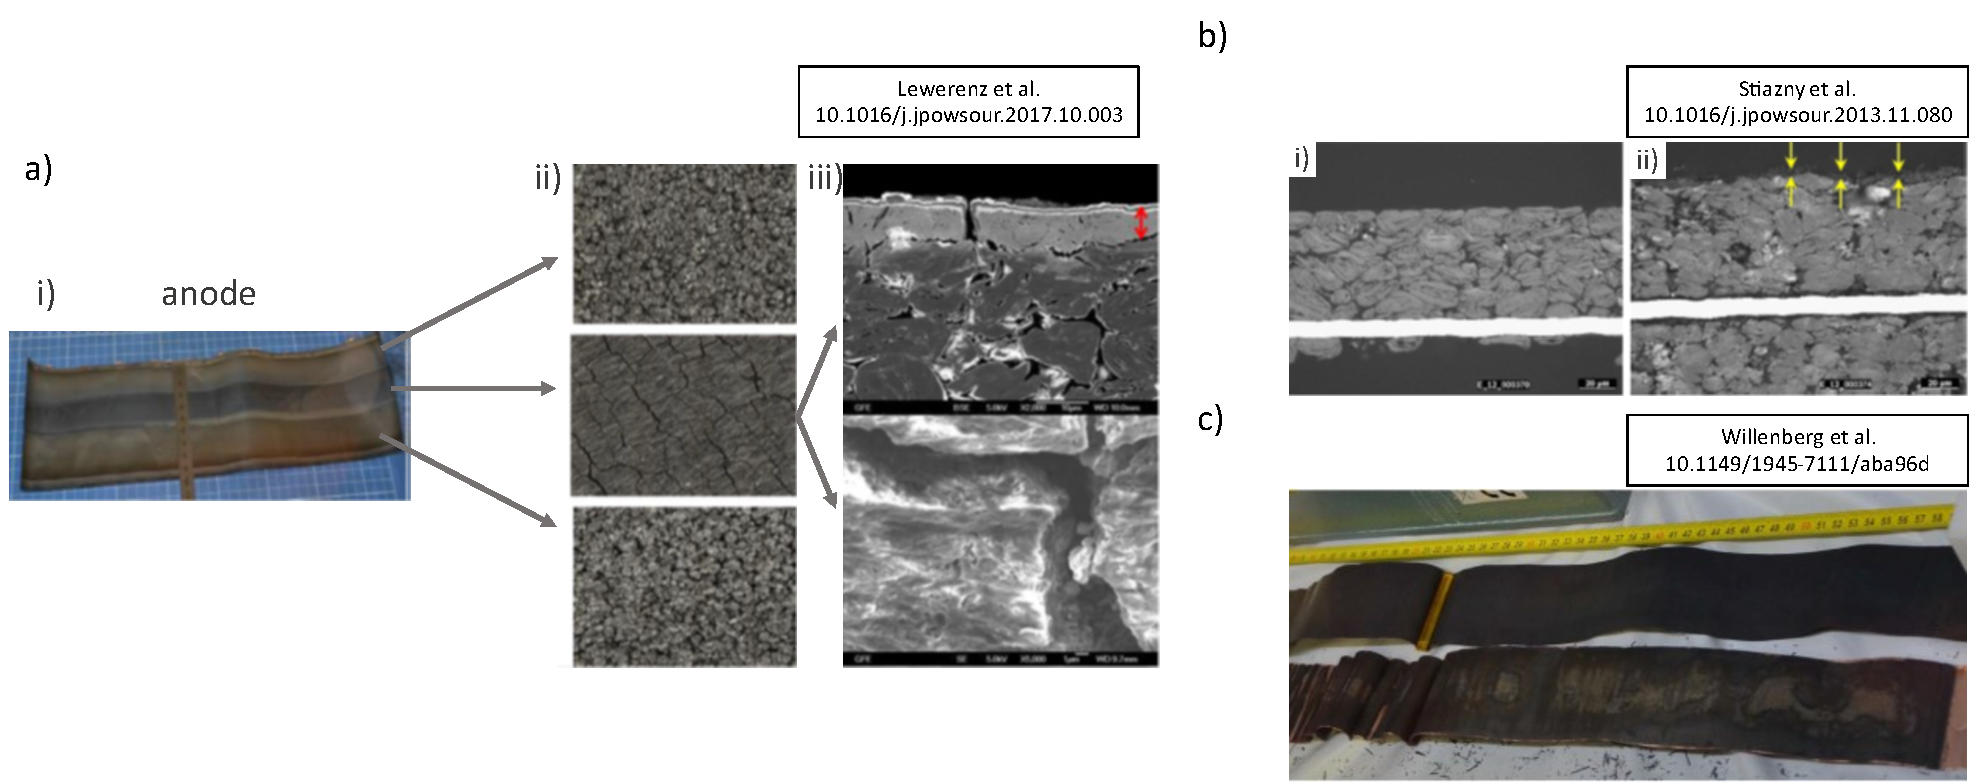
\includegraphics[scale = 0.5]{figures/CoveringLayers.pdf}
\caption{``Covering layers'' as found via post-mortem analysis in cells with knees. Covering layers are commonly observed in cells with knees but are a poorly understood source of active material loss.
a) A covering layer in the middle of the anode of an unwound cylindrical cell, along with laser microscope images of top, middle and bottom sections and scanning electron microscopy images of the middle section with a covering layer. The red arrow corresponds to a thickness of $10 \mathrm{\mu m}$. Reproduced with permission from Lewerenz et al. \cite{lewerenz_post-mortem_2017} Copyright 2017, Elsevier. b) Covering layer in the middle of the anode of an unwound cylindrical cell. CC-By Willenberg et al. \cite{willenberg_development_2020}. c) Scanning electron microscopy cross-sections of new and aged electrodes with a visible covering layer. Reproduced with permission from Stiaszny et al. \cite{stiaszny_electrochemical_2014} Copyright 2014, Elsevier.}
\label{fig:covering_layers}
\end{figure}

On the macroscale (cell level), both the external pressure (for pouch and prismatic cells) and internal jellyroll deformation (for cylindrical cells) can impact cell lifetime. Pouch and prismatic cells either without external pressure\cite{wunsch_investigation_2019} or with high external pressure\cite{cannarella_stress_2014} can show rapid knees, indicating a ``sweet spot'' to avoid a knee and maximize lifetime. Cannarella et al.\cite{cannarella_stress_2014} also found that the surface layer is more pronounced with increasing external pressure.
For cylindrical cells, several studies showed jelly roll deformation in cells at their end of life as also shown in (Figure \ref{fig:covering_layers})\cite{willenberg_development_2020, willenberg_high-precision_2020}. Carter et al. proposed this even as the primary degradation mode in madrel-free 18650 cells operated at 0 °C \cite{carter_mechanical_2019}.
Kok et al. \cite{kok_virtual_2019} could show the formation of a covering layer through virtually unrollying the jelly roll directly from CT data without post-mortem analysis.
In addition  CT studies by Pfrang et al.~\cite{pfrang_long-term_2018} revealed jelly roll deformation using cells from Ecker et al. \cite{ecker_calendar_2014}. Threshold mechanism?

\pbox{Philipp, can you add more citations and discussion here? I was expecting more than 1 sentence on jelly roll deformation :)}

\subsection{Interactions and heterogeneity}

\pbox{This will be a new section discussing how everything's really complicated}

While the six knee pathways we have identified can occur independently, these pathways can clearly interact. For instance, loss of active material plays a central role in four of our six pathways. This coupling between degradation mechanisms can create positive feedback mechanisms, as explored by X et al. with a single-particle model. These interactions can also occur across length scales (figure X), as SEI growth on the nanometer level can drive lithium plating on the centimeter level.
Given the high sensitivity of snowball pathways to small changes in state, interacting knee pathways can create “leveraged” pathways with immense sensitivity to changes in state.

As an extreme example of coupling between knee mechanisms, consider a hypothetical “quadruple snowball” based on previously identified mechanisms. First, particle cracking leading to loss of active material can snowball since the current on the remaining active particles is continuously increasing, driving additional mechanical stress. Second, loss of active material itself can snowball with percolation-limited connectivity (i.e., if the active material fraction drops below the critical percolation threshold). Third, loss of active material from the negative electrode can cause kinetic lithium plating to snowball, since the local current density will keep rising on the remaining active material, increasing the driving force for lithium plating over reversible interaction. Lastly, lithium plating can exhibit a snowball due to its nucleation and growth kinetics. While contrived, feedback between multiple knee pathways is perhaps probable given the shared sensitivities of many of these pathways. 

Electrochemical, thermal, or mechanical heterogeneity within a cell may also exacerbate these knee pathways....

In short, the impact of interactions and heterogeneity on knee pathways is poorly understood and an opportunity for future work. 

Interactions 
This section addresses the coupling between different knee mechanisms and pathways which could either occur simultaneously or trigger other mechanisms. 
Dizzying array of degradation mechanisms

Many vicious cycles :(

LAM plays a central role
Loss of active material of NE for lithium insertion is caused mainly due to particle cracking and electrical contact loss/blockage of active sites by resistive surfaces. Lithium trapped inside isolated graphite particles can contribute to cell capacity decrease due to unavailability to cycle.
Multi length scale interactions (mechanics, DCR, etc)

Heterogeneity

Commercially-relevant form factors have thermal, mechanical, electrochemical gradients 
K.Jalkanen et al \cite{jalkanen_cycle_2015} showcased cyclic aging at different cycling temperatures (\SI{25}{\celsius}, \SI{45}{\celsius} charge and \SI{65}{\celsius} discharge) through capacity fade. At temperatures above \SI{60}{\celsius}, aging at NE (graphite electrodes) is different compared to low temperature aging. Elevated temperatures contribute to excess Li plating during  cycling apart from the SEI-layer increase on anode surface which occurs during normal charging and discharging cycles at room temperature. Increase in SEI-layer thickness enhances graphite electrode polarization leading to additional plating. SEI-growth also leads to electrolyte consumption due to prolonged cycling at high temperatures. Irreversible lithium plating reduces graphite electrical contact, when lost, results in isolated dead lithium and capacity degradation \cite{petzl_lithium_2015}.  

Pressure Gradients
Bach et al.\cite{bach_nonlinear_2016} applied a hose clamp around the circumference of an 18650 cylindrical cell, and a post-test teardown clearly showed lithium plating localized to the regions of the electrodes that were under compressive stress. From this test, the authors concluded that internal gradients in pressure induced by the current-collecting tab can also cause lithium plating. Coin cell and pouch cells are also sensitive to localized external pressures. Fuchs et al \cite{fuchs_post-mortem_2019} applied an external pressure of 20MPa using a stainless steel sphere to a pouch cell while cycling it. They observed a ring of localized plating on the anode, which they attributed to pore closure causing increased local current density (and resulting increased local overpotentials). Additionally, the cathode particles in the pressurized region were crushed, leading to exposure of additional active material surfaces to the electrolyte thus enhancing degradation. Liu et. al introduced "defects" consisting of a compressed separator (such that pore closure occurred) of different shapes to study their effects on plating. They showed that larger defects induce higher probabilities of plating. They also performed simulations of these defects, which showed regions of anode potential below the Li/Li+ nucleation barrier (agreeing with experiments). They also showed that defect shape can influence the plating patterns. \cite{liu_size_2018} Okasinski et. al showed that the design of coin cells can lead to these sorts of heterogeneity and increases in plating patterns \cite{okasinski_situ_2020}


canarella \cite{cannarella_stress_2014}

\cite{liu_size_2018, okasinski_situ_2020}
Cell design (cylindrical cell gradients, tab pressure)

Usage
Thermal transients \cite{carter_detection_2019}
Apart from the main mechanisms causing knees due to plating, few other causes are based on substantial and mild temporally thermal transient conditions lead to a rapid capacity fade in cells when compared with cells at a fixed equilibrium temperature. Temporal transient thermal gradients (40 \degree C to 0 \degree C) also contribute to Li ions being plated as Li instead of intercalation, which accelerates capacity fade over subsequent cycles causing knees and ultimately resulting in jellyroll collapse. Carter 2019 tested two sets (equilibrium and transient cells) at different temperatures (at 40 \degree C, 20 \degree C, 0\degree C) to understand thermo-electrochemical coupling. Equilibrium cells at 40 \degree C and 20 \degree C show minimal degradation while equilibrium cell at 0 \degree C has initial minimal degradation, then a gradual decay midway. Transient cells demonstrate high lithium stripping at initial discharge cycles due to thermal transient causing anode thickness increase, pressure buildup in jelly roll resulting in plating and capacity loss. \fbox{Figure \ref{fig:knee_definition}}  highlights the difference between the 0 \degree C and Transient 40 \degree C to 0 \degree C jellyroll collapsing behaviors. Primary reason for degradation is jellyroll collapse for 0 \degree C cell while the rapid lithium plating followed by jellyroll collapse causes capacity fade knee point in Transient 40 \degree C to 0 \degree C cell.         
Hotspots

\section{Factors influencing the knee}

\pbox{I haven't edited this yet}

We surveyed the literature to identify empirical case studies in which the knee point can be controlled via changes to a single variable. Table S1 classifies these case studies into three categories based on the nature of the variable: cell design, testing conditions, and sampling/testing variability (a special case of these two categories). Some testing conditions have a consistent impact on the emergence of the knee; for example, higher charging rates and wider cycling voltage ranges accelerate the appearance of the knee. However, the impact of other variables (e.g., discharging rate and rest times) is less clear and may depend on the specific cell design and operating conditions.

\subsection{Cell design}

While the dependence of knees on cell usage conditions has been studied extensively, less attention has been focused on the dependence of knees on cell design---likely due to the challenges of lab-scale cell fabrication. Ma et al.\cite{ma_editors_2019}, one of the most comprehensive works on this topic, studied the impact of various electrodes and electrolytes on the location of the knee, finding that cathode particle coatings and low cathode loadings delayed the knee. These knees were classified as resistance ``pseudo-knees'' due to increased electrolyte oxidation on the cathode, as evidenced by the strong dependence of the knee severity on discharge rate as well as cathode impedance measurements. Ma et al. al.\cite{ma_editors_2019} and Glazier et al.\cite{glazier_analysis_2017} also found that the graphite type (i.e., natural or artificial) substantially impacts the knee location, though the root cause of the knee in this case is unclear(PETER TO EXPLORE FURTHER).

Electrode loadings---specifically, anode loadings---can also lead to knees via the lithium plating pathway.
If the electrode is too thin or the capacity is too low, thermodynamic plating can occur; however, kinetic plating can occur if the electrode is too thick. (LI PLATING TEAM--WHAT ARE GOOD REFERENCES FOR THESE?)

Additionally, small changes in the electrolyte can play an outsized role on the lifetime performance. Ma et al.\cite{ma_editors_2019} demonstrated the sensitivity of the knee location to the electrolyte additive package; specifically, high methyl acetate (MA) concentrations (MA is used to increase electrolyte transport capability) and low LiPF$_6$ concentrations consistently lead to earlier knees. These knees were attributed to increased electrolyte oxidation on the cathode. Ma et al.\cite{ma_editors_2019} also identified other electrolyte systems with a strong knee sensitivity. Additionally, as previously discussed, additive depletion (e.g., FEC depletion in cells with high silicon content in the anode) can be a direct cause of knees for some cell designs.

Lastly, mechanical deformation knees are naturally highly sensitive to the cell form factor. For instance, deformation of the core(PHILIPP -- WHAT PAPERS TO CITE?) can only occur in cells with cores, namely cylindrical cells.

\subsection{Testing conditions}

\subsubsection{Charging rate}
Increasing the charging rate has accelerated the onset of the knee-point across a range of batteries. \cite{lewerenz_systematic_2017,lewerenz_post-mortem_2017, petzl_lithium_2015, burns_-situ_2015, waldmann_optimization_2015, schuster_nonlinear_2015, severson_data-driven_2019, schindler_fast_2018, keil_linear_2019}. However, the critical charging rate leading to knee-onset varies substantially, with knees appearing at C-rates as low as 1C \cite{waldmann_optimization_2015} and as high as 8C \cite{lewerenz_systematic_2017}. 

Higher charging rates advance the knee point via Li plating and accelerated SEI growth. Either Li plating or SEI growth may directly cause knee onset, but knee onset is also attributed to pore clogging caused by either or both of these mechanisms \cite{yang_modeling_2017}. It is difficult to distinguish these causes, even in cases with detailed post-mortem characterization. Key evidence for both Li plating and accelerated SEI growth driven by increased charging rate is found in a series of papers by Lewerenz et. al., examining the aging of cylindrical 8 Ah LFP/Gr cells \cite{lewerenz_systematic_2017,lewerenz_post-mortem_2017}. They present evidence demonstrating that knees reliably occur across a set of test replicates at 8C charging rate, while knees may occur less reliably at charging rates as low as 2C. Evidence of Li plating after knee onset driven by increased charging rate was also confirmed by Petzl et. al. \cite{petzl_lithium_2015} and Burns et. al. \cite{burns_-situ_2015}. 



\subsubsection{Discharging rate}

Unlike charging rate, the effect of discharging rate on the knee point is mixed (Figure X).
In some systems, an increased discharging rate
accelerates the knee onset.
Omar et al.\cite{omar_lithium_2014} found that a higher discharging rate (1C to 15C) accelerated the knee for cylindrical LFP/graphite cells.
Diao et al.\cite{diao_accelerated_2019} showed no effect of discharge rate except at 60°C, where the cells discharged at 2C degraded almost twice as quickly as the cells discharged at 0.7C or 1C.
High discharging rates can lead to worse cycle life due to higher temperatures, which accelerates electrolyte reduction (i.e., SEI growth) and electrolyte oxidation (i.e., cathode resistance growth). Additionally, high discharging rates can lead to ``pseudo-knees'' when the resistance growth or lower cutoff voltage is high.

In other systems, an increased discharging rate can delay the onset of the knee.
Atalay et al.\cite{atalay_theory_2020} found that reducing the discharge rate from 4C to 1C accelerated the knee for 18650 NCA/graphite cells.
Keil et al.\cite{keil_charging_2016} illustrated how discharging current had no effect on LMO+NMC/graphite and LMO+LCO/graphite cylindrical cells, but a lower discharging current (3A, 2.7C) led to faster degradation than a higher discharging current (5A, 4.5C) for an LFP/graphite cylindrical cell when charged at 4.5C; they did not identify a mechanism. 
Similarly, Keil et al.\cite{keil_linear_2019} found that increasing discharging current from 1C to 2C led to the elimination of the knee in NMC/graphite cylindrical cells.
While more work is needed to understand these results, one hypothesis for these observations is decreased calendar aging for cells with faster discharge rates.
In other words, cells with less time spent cycling simply have less calendar aging. This hypothesis does suggest a sensitivity of the x axis to the apparent severity of the knee; for instance, plotting capacity retention vs. time instead of cycle number may decrease the apparent severity of the knee.

\subsubsection{Voltage limits} 
A wider voltage window generally accelerates the onset of the knee point \cite{ecker_calendar_2014, pfrang_long-term_2018, klett_non-uniform_2014, ma_novel_2019, petzl_lithium_2015, schuster_nonlinear_2015}. In one of the broadest studies, Ecker et al. \cite{ecker_calendar_2014} considered six DODs (100, 80, 50, 20, 10, and 0.5 \%) with up to six voltage windows per DOD. They found that the EFC systematically decreased with increased DOD. By 1000 EFC, all cells with DODs greater than 25-75 \% had a capacity below 80 \% and showed a knee point. When varying the voltage window at the same DOD, the authors observed the highest degradation in cells cycled at low and high SOCs; the lowest degradation was observed for a midpoint SOC of 50 \%. Accelerated degradation at extreme SOCs was also observed in other studies \cite{aiken_accelerated_2020,ma_novel_2019, zhu_investigation_2021}.

The impact of the voltage window on knee point onset is typically attributed to resistance growth stemming from enhanced expansion and cracking of the electrode during intercalation. In several studies, capacity knees have aligned perfectly with resistance knees \cite{ecker_calendar_2014, klett_non-uniform_2014, schuster_nonlinear_2015, zhu_investigation_2021}. High voltages may also drive electrolyte oxidation at the cathode \cite{aiken_accelerated_2020} and for some cathodes, active material loss via Mn dissolution \cite{ma_novel_2019}. 



\subsubsection{Rests}

The effect of rests during cycling on the knee occurrence is mixed. 
Keil et al.\cite{keil_linear_2019} found that decreasing rest time at both the top of charge and the bottom of discharge from 900 seconds to 10 seconds delayed the knee point in graphite/NMC cylindrical cells.
Ma et al.\cite{ma_editors_2019} found an identical result: removing the 30-minute rests at both top-of-charge and bottom-of-discharge delayed the knee, but only with an upper cutoff voltage of 4.3 V. The rest time had no effect at 4.1 V.
These observations were rationalized by less time at high potential when plotted as a function of cycle number.
In contrast, Epding et al.\cite{epding_investigation_2019} found that longer rest times between cycles delayed the knee occurrence. The authors proposed that this rest offered reversibly plated lithium time to reintercalate; another possibility is that the rest allowed for greater utilization of cycleable lithium(cite Rashid Gupta, see comment). More generally, increased rest periods may delay the onset of knees driven by high overpotentials (e.g., kinetic lithium plating at high rates or low temperatures) but may exacerbate the onset of knees driven by side reaction product buildup (e.g., porosity decrease, cathode resistance growth, etc)---particular for rests at high state of charge. In general, more work is needed to understand the sensitivity of knees to rest at both low and high state of charge.


\begin{figure}[ht]
\centering
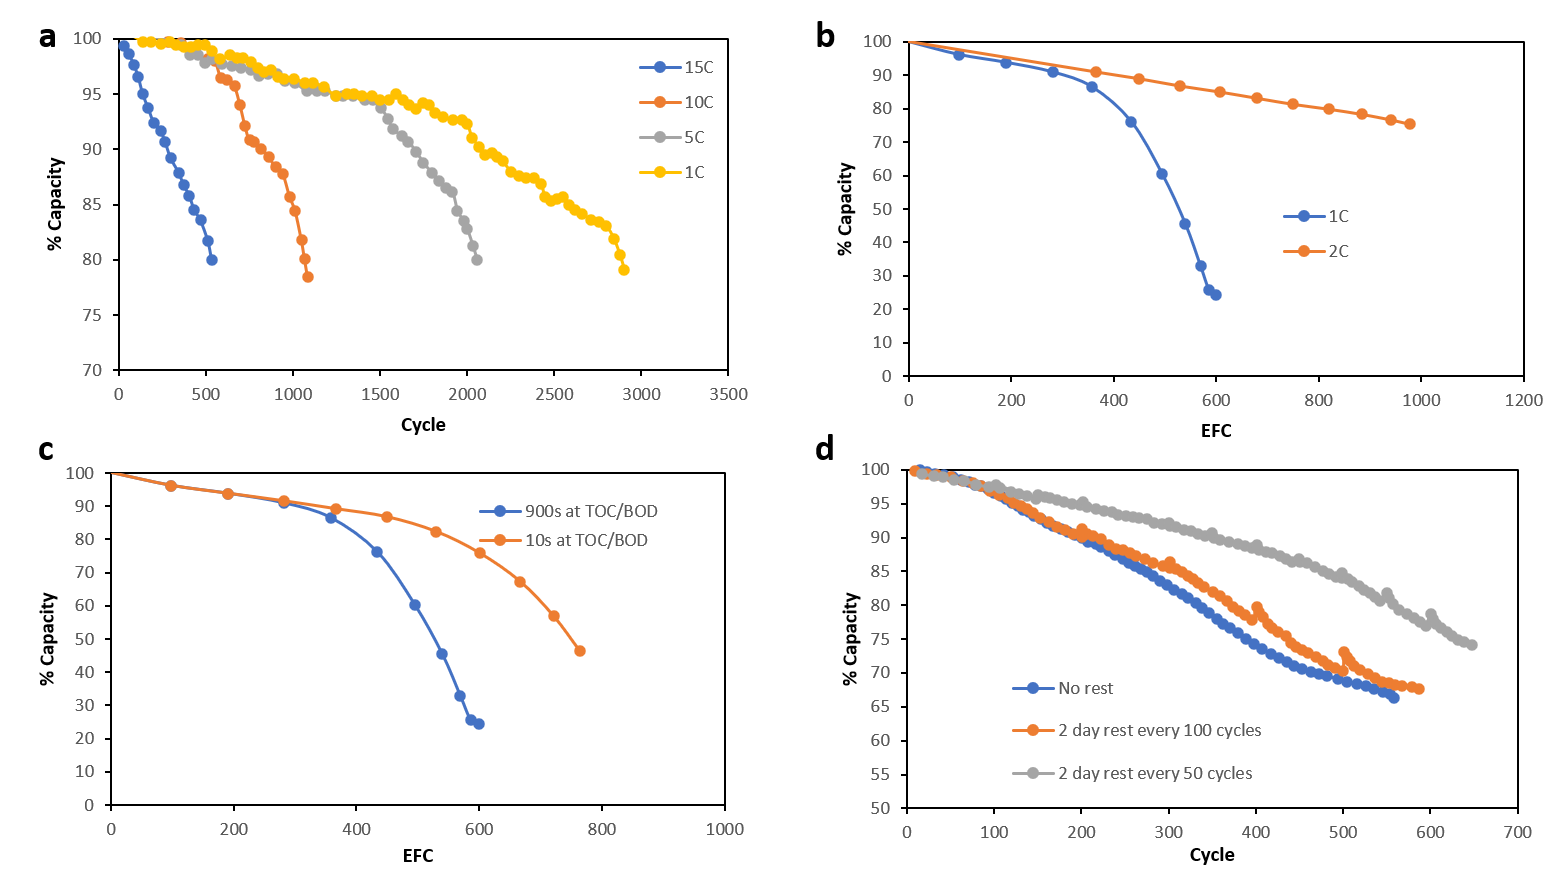
\includegraphics[scale = 0.6]{figures/Discharge-rest_cycle.png}
\caption{Discharge rate and rest time have mixed effects on knee point onset depending on the testing conditions. (a) Higher discharge rate accelerates knee onset. Adapted from \cite{omar_lithium_2014} (b) Lower discharge rate accelerates knee onset. Adapted from \cite{keil_linear_2019} (c) Longer rest time accelerates knee onset. Adapted from \cite{keil_linear_2019} (d) Shorter rest time accelerates knee onset. Adapted from \cite{epding_investigation_2019}. To isolate the influence of calendar aging, the above are replotted with a time axis in the Supporting Information.  }
\label{fig:discharge-rest_cycle}
\end{figure}


\subsubsection{Temperature}
The effect of temperature on knee onset depends on the test conditions. For example, some studies have found that knee onset is accelerated at temperatures above or below 25 degrees Celsius \cite{zhang_accelerated_2019, waldmann_temperature_2014, waldmann_optimization_2015} or 35 degrees Celsius \cite{schuster_nonlinear_2015}. In general, the temperature of minimal degradation is lower for LFP cells than NMC cells \cite{preger_degradation_2020}. 

There is no straightforward dependence on temperature because different mechanisms dominate in different temperature ranges (Figure \ref{fig:temperature_and_pressure}). At lower temperatures, the acceleration of the knee point is attributed to Li plating. At elevated temperatures, knee point onset is driven by SEI growth \cite {zhang_accelerated_2019,schuster_nonlinear_2015,waldmann_temperature_2014,waldmann_optimization_2015}.

\subsubsection{Pressure}
Studies of pressure dependence in pouch and prismatic cells have demonstrated 'sweet spots' for optimal performance. The knee point can be accelerated by either an absence of pressure or excess pressure. For example, Wünsch et al. increased the cycle life of 37 Ah commercial NMC pouch cells from 500 (no bracing) to 3200 (optimal spring compression) while investigating various methods of bracing \cite{wunsch_investigation_2019}. Figure \ref{fig:temperature_and_pressure} shows another example from Cannarella et al. for an LCO pouch cell \cite{cannarella_stress_2014}. Even in a cylindrical cell, heterogeneous compression in the test fixture can accelerate the knee point \cite{bach_nonlinear_2016}. 

For pouch and prismatic cells, some applied pressure is needed to enhance conductivity and particle contact. When too much pressure is applied, high mechanical stress is not always evenly distributed throughout the cell. This causes heterogeneous delamination, surface film formation, and uneven Li distribution (Li plating). Li plating was also reported in cylindrical cells that experienced heterogeneous compression from test fixtures \cite{bach_nonlinear_2016}. 

\begin{figure}[ht]
\centering
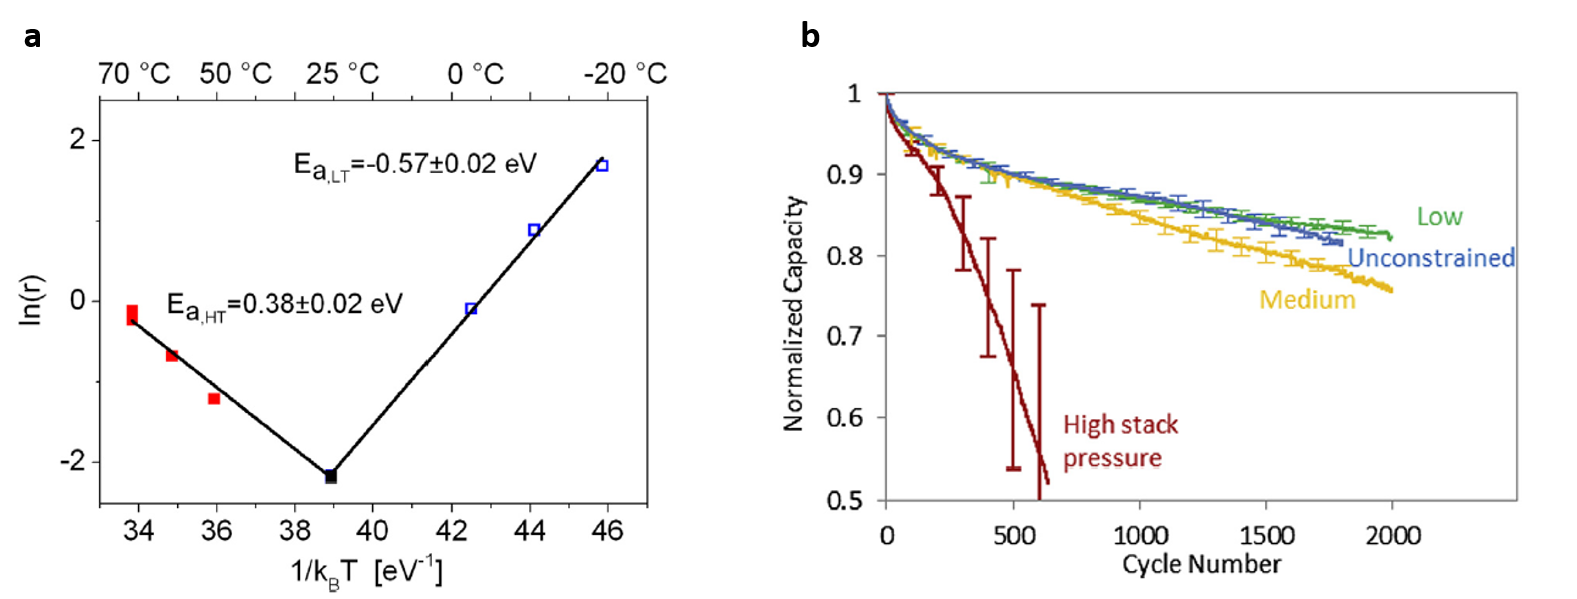
\includegraphics[scale = 0.6]{images/Temperature_and_pressure.png}
\caption{Transition in degradation mechanism based on (a) environmental temperature and (b) applied pressure, illustrating a ``sweet spot'' for each variable. Adapted from Waldman et al.\cite{waldmann_temperature_2014} and Cannarella and Arnold\cite{cannarella_stress_2014}, respectively.}
\label{fig:temperature_and_pressure}
\end{figure}



\subsection{Sampling and testing variability}

Nominally identical cells cycled identically often show differences in knee behavior. This sampling variability includes both intrinsic variability from manufacturing (component-level variation, cell assembly, etc.) and extrinsic variability from testing (cycler calibration, temperature control, etc.). These sources of variability cannot be distinguished.

The magnitude of sampling variability is a function of the cell design, manufacturing variability, and testing conditions. Sampling variability may increase with more aggressive cell designs (e.g., higher silicon content), more manual cell assembly processes, and more aggressive testing conditions (particularly for test setups with no or poor temperature control). The magnitude of sampling variability can be estimated using studies with fairly large sample sizes (i.e., at least $\sim$10 cells). Baumhöfer et al.\cite{baumhofer_production_2014} and Harris et al.\cite{harris_failure_2017} studied this type of variation in 48 cells and 24 cells, respectively, finding widely varying knee locations across their datasets. These studies did not identify a correlation between beginning-of-life capacity and end-of-life capacity, suggesting that the underlying state variables controlling the knee location did not manifest in the initial capacity measurements. In general, sampling and testing variation also pose challenges for accurate knee prediction; we recommend identifying the manufacturing and testing variation of the state variable of interest in evaluating the accuracy of knee prediction methods. Beck et al.\cite{beck_inhomogeneities_2021} provide a detailed review of cell-to-cell variation.

\section{Modeling and predicting knees}

\pbox{Anyone interested? I think a key message here is which pathways/types of pathways can be predicted theoretically and with measurements}
\newline
\ssri{I think this would be really valuable because predicting knees is really the economic value addition from all the knee point analysis. We spoke a little bit about how ML could predict knees -- given how much we've talked about pathways (also as mentioned by Peter above), I think there is a point to be made about physics-inspired/physics informed ML i.e., an ML framework coupled with an electrochem model which is one of the few ways in which something about the pathways can also be said in addition to the ML predicted knee. Goes a long way in making falsifiable ML models wrt knees.}


Recently, joint prediction of capacity and internal resistance  trajectory degradation for was carried out in \cite{strange_prediction_2021}

\subsection{Empirical relationship between capacity knees, resistance elbows, and end-of-life}

Predicting knees is important but predicting end-of-life is more directly relevant for product performance and estimating warranty costs. Thus, we explored empirically the linear relationship between knee locations and end-of-life across 15 datasets (306 cells) -- \gbox{refer to Yulia's table}.

\begin{figure}[ht]
\centering
% \begin{subfigure}{.5\textwidth}
%   \centering
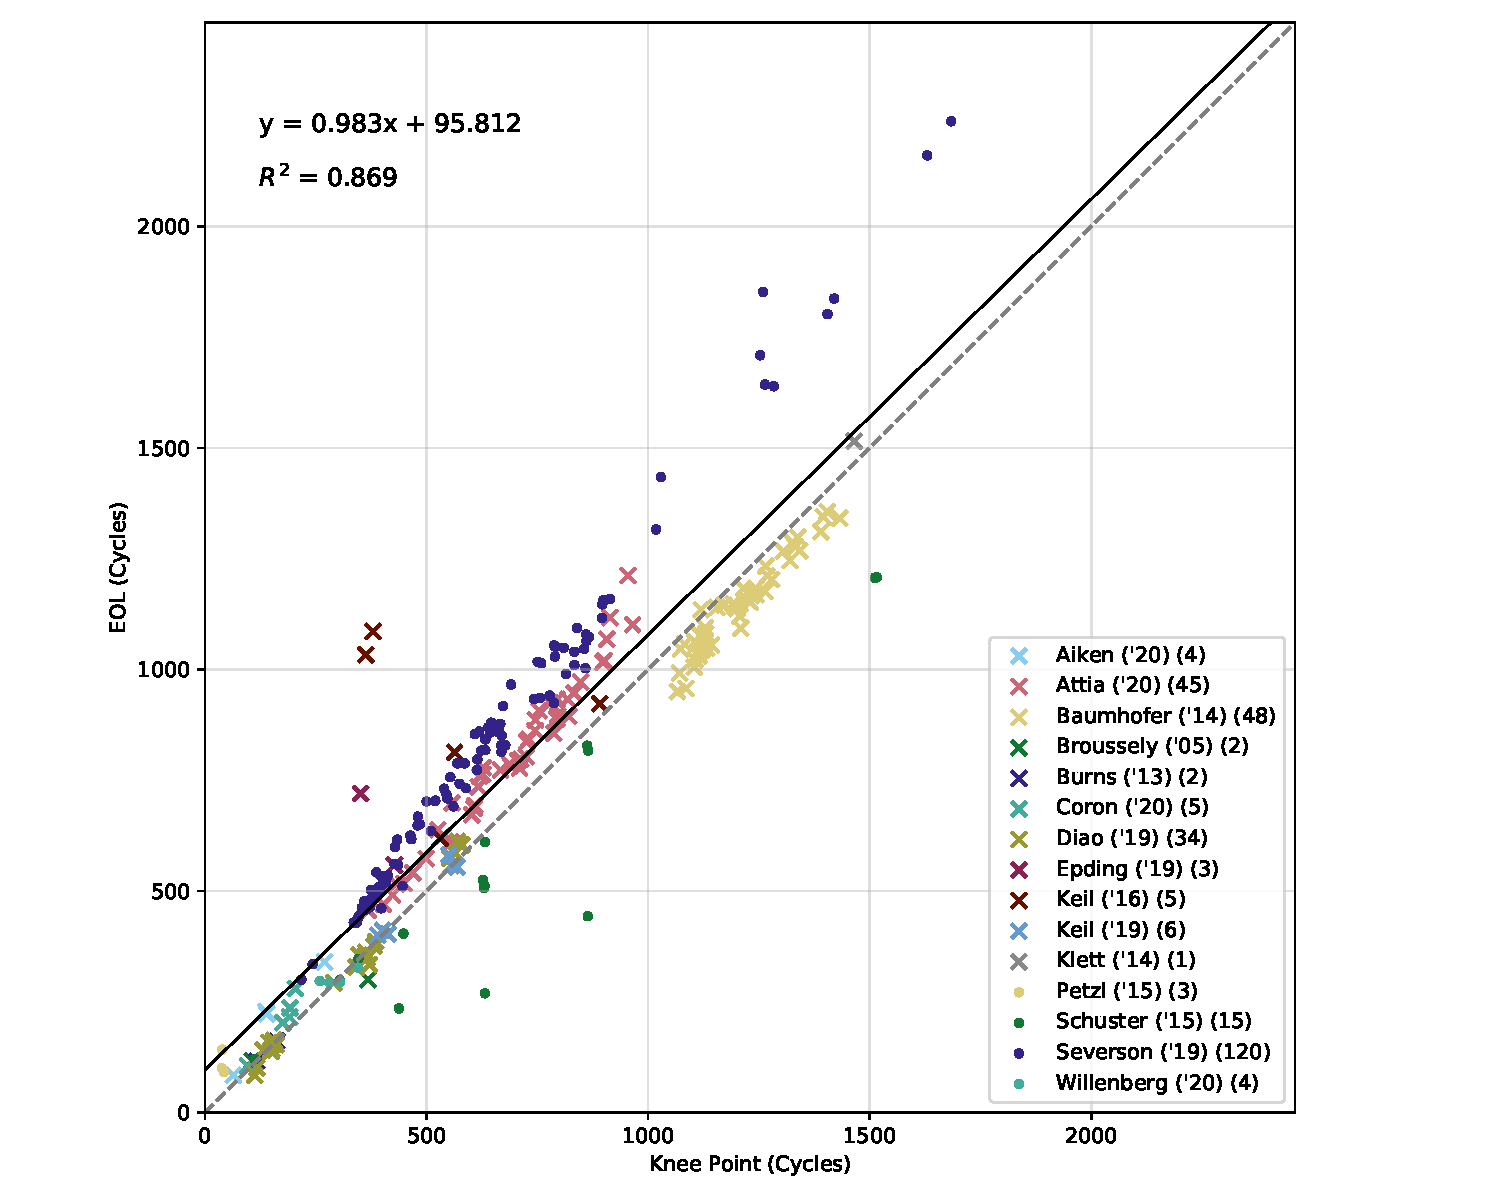
\includegraphics[scale=0.70]{figures/AcrossDatasetsknee-to-EOL}
%   \caption{Linear regression of knee-point to EOL point}
  \label{fig:kneepoint2EOL}
% \end{subfigure}%
\caption{Total of 306 cells across 15 datasets. The knee identification algorithm employed is the Bacon-Watts one. Linear relation between knee-point and EOL (defined as 80\% capacity).}
\label{fig:knees2EOL}
\end{figure}

This observation is supported by the fact that many aging studies have shown that capacity knee onset is nearly always correlated to the onset of rapid resistance growth, across different cell chemistries, architectures, and test protocols. The relative capacity and resistance at the knee onset point from several studies that reported both capacity fade and resistance growth are reported in Table \ref{tab:dcr_growth_papers}. Of all these aging studies, cells with capacity knees always displayed resistance elbows, and with the exception of the work by Martinez-Laserna et al \cite{martinez-laserna_technical_2018}, the reverse is also true. One assumption used in the model shown in Fig. \ref{fig:dcr_knee} but not reflected in these results is that linear resistance growth continues after knee onset; in much of the experimental work, regardless of the remaining capacity or relative resistance growth at knee onset, the previously linear resistance growth suddenly accelerates, leading to a resistance elbow as well. This is likely because many of the resistance growth and capacity fade mechanisms are intertwined. For instance, SEI growth causes both an increase in cell resistance as well as a decrease in available lithium, while loss of electrode active material may cause stoichiometric shifts of lithium while also decreasing available surface area for electrode-electrolyte reactions and thereby increasing cell resistance as well.

\begin{figure}[ht]
\centering
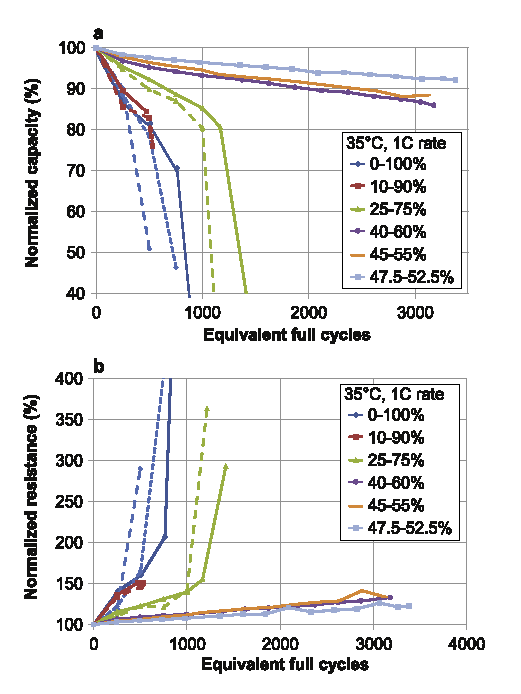
\includegraphics[scale=1.0]{figures/ecker_capacity_vs_dcr.eps}
\caption{Correlation between capacity knees and ``resistance elbows''.
(a) Normalized capacity and (b) normalized resistance vs. equivalent full cycles for cells cycled at 1 C and 35$^{\circ}$C.
Different cycle depths around a mean SOC of 50\% are compared. Each trend displays a single cell. The correlation between capacity knees and resistance elbows is evident.
Adapted from Figure 12 of Ecker et al.\cite{ecker_calendar_2014}
}
\label{fig:ecker_capacity_and_resistance}
\end{figure}

\newgeometry{margin=2.5cm} % modify this if you need even more space
\begin{landscape}

\begin{table}[!ht]
    \centering
    \begin{tabular}{||c||c|c|c|c||}
        \hline
        Reference & Multiple test conditions? & Test replicates? & Rel.~capacity at knee onset & Rel.~resistance at elbow onset \\
        \hline
        Ecker et al.\cite{ecker_calendar_2014} & Yes & No & 80\% & 150\% \\
        Rahe et al.\cite{rahe_nanoscale_2019} & No & No & 90\% & 160\% \\
        Willenburg et al.\cite{willenberg_development_2020} & No & Yes & 90\% & 120\% \\
        Broussely et al.\cite{broussely_main_2005} & No & Yes & 70\% & 200\% \\
        Schuster et al.\cite{schuster_nonlinear_2015} & Yes & No & 80\% & 300\% \\
        Lewerenz et al.\cite{lewerenz_systematic_2017, lewerenz_post-mortem_2017} & Yes & Yes & 80\% & 110\% \\
        Martinez-Laserna et al.\cite{martinez-laserna_technical_2018} & Yes & No &  85\% & 170\% \\
        Braco et al.\cite{braco_experimental_2020} & No & Yes & 70\% & 200\% \\
        Frisco et al.\cite{frisco_understanding_2016} & No & No & 80\% & 200\% \\
        Klett et al.\cite{klett_non-uniform_2014} & No & No & 80\% & 110\% \\
        Pfrang et al.\cite{pfrang_long-term_2018} & No & Yes & 75\% & 130\% \\
        Wunsch et al.\cite{wunsch_investigation_2019} & Yes & No & 95\% & 100\% \\
        \hline
    \end{tabular}
    \caption{Summary of studies reporting both capacity and resistance over cell lifetime with capacity knees and/or resistance elbows. All studies measure resistance using a direct-current pulse except for Schuster et al. \cite{schuster_nonlinear_2015}, which uses EIS. Relative capacity and resistance values at capacity knee/resistance elbow onset are estimated either from a single measurement or roughly averaged from several measurements.}
    \label{tab:dcr_growth_papers}
\end{table}

\end{landscape}
\restoregeometry

\subsection{Modeling approaches}
In this section we discuss the different approaches found in the literature to model the knee. Note that we have constrained to only those articles which explicitly show a knee arising from the model, so there might be other models not included in this review which could show also a knee. For clarity, we group the different models depending on whether their underpinning electrochemical model is an empirical, equivalent-circuit, or physics-based. The models are also summarized in Table {\color{red} CROSSREF}. Empirical models are usually standalone, while both equivalent-circuit and physics-based must be coupled to an electrical/electrochemical model. This coupling goes both ways: the electrochemical model informs the degradation model, and the degradation model alters some of the electrochemical model parameters to account for the degradation. 

First we focus on empirical models. These models use empirical laws to describe the evolution of the battery capacity with cycling number, and their parameters need to be calibrated with experimental data. They are usually not coupled to an electrical/electrochemical model and therefore they cannot provide a voltage response. Smith et al. \cite{smith_models_2014,smith_life_2017} propose an approach that consists on defining the total capacity of the battery as the minimum of multiple capacities, each associated to a particular degradation mechanism. Hence, this is a hidden mechanism. On the other hand, Diao et al. \cite{diao_accelerated_2019} propose an equation for the normalized capacity that follows a power law for cycle number and an exponential for temperature. The combination of the two power laws captures the knee, while the exponential in temperature adjusts the capacity curve to different temperatures. This is again a hidden mechanism, where one power law has very small contribution at early times but ends up dominating, causing the knee to appear. Finally, Pugalenthi et al. \cite{pugalenthi_piecewise_2020} propose a mechanism in which the model switches from a linear to an exponential behavior at a given time, and the latter captures the knee. This is an example of a threshold triggered by reaching a given cycle number.

The next type of model to consider are equivalent-circuit models. These models represent the battery by an equivalent electrical circuit the parameters of which are determined by fitting to experimental data. These models, even though do not provide information on the internal states of the battery, can produce very accurate predictions of the battery behavior when properly calibrated. The degradation effects are then introduced by varying these model parameters. Anse\'an et al. \cite{ansean_operando_2017} study an equivalent-circuit model including LAM and LLI, the latter induced by lithium plating, based on the \emph{'alawa} framework\cite{dubarry_synthesize_2012}. Another approach, suggested by Mandli et al.,\cite{mandli_analysis_2019} uses a very simple equivalent circuit model and, by varying the maximum capacity and the internal resistance captures the knee. In both cases, the knee is caused by a hidden mechanism. Note that this type of models, even though they can provide very accurate results, do not provide much insight on the physics behind the degradation modes.

Finally, we consider the physics-based models. There are numerous possible combinations of electrochemical and degradation models, including combinations of multiple degradation effects, which can yield different types of degradation curves.\cite{reniers_review_2019} After reviewing the literature, we have found that the different degradation models that show a knee can be grouped in three types. The first type includes lithium plating, SEI growth and pore clogging; the second type includes SEI growth, loss of active material and particle fracture; while the last type includes SEI growth, loss of active material and electrode. The first type, which is a snowball effect mechanism, is the one the has been investigated the most \cite{yang_modeling_2017,yang_understanding_2018,muller_model-based_2019,atalay_theory_2020,keil_electrochemical_2020}. At the early cycles, only SEI growth occurs, which yields a linear aging. However, the SEI growth triggers a decrease in the anode potential which, after some cycles, triggers the lithium plating which causes the knee. The second type has two examples. Lin et al. \cite{lin_comprehensive_2013} also include manganese plating and they find that the knee is caused by the narrowing of the anode SoC operating window, which is a hidden mechanism. On the other hand, Reniers et al. \cite{reniers_review_2019} propose many different combinations of aging mechanisms but here we focus on SEI growth + LAM + particle fracture as it is the one that shows a knee, which is caused by a snowball effect produced by the interaction of the different mechanisms. The last mechanism, proposed by Kupper et al.,\cite{kupper_end--life_2018} includes is similar to the previous one but is has electrode dry-out instead of particle fracture. The knee is caused by the deactivation of graphite, which is a hidden mechanism, as depending on the activity-saturation relationship the knee is present or not.

As mentioned earlier, in this section we have only discussed the models from articles that showed the presence of a knee, and it is likely that other existing models could also show knees. However, from reviewing the literature we can conclude there is still a lot of modeling work to be done when it comes to modeling the knee, especially on physics-based models. Most of the efforts have been focused on modeling the combined effects of lithium plating, SEI growth and pore clogging. On the other hand, other models including SEI growth, loss of active material and either particle fracture or electrode dry-out have also been proposed, but they have been less studied. For all cases, there are multiple future areas of research, but here we suggest three. The first one is to understand the path leading to the knee for each model, clarifying if a subset of the effects can still cause the knee. Finding the minimal models that lead to a knee would allow us to better understand the nature of the phenomenon and how to prevent it. The second area for further research is on the parametrization of these models so they can be used to predict the behaviour of real batteries. The last area is the development of new models, both models accounting for other degradation mechanisms but also simplified models that can be simulated efficiently.

Another aspect to consider would be the degradation effects at the macroscale. The effects discussed here posed at the microscale, that is over a single layer of the battery. However, accurately capturing macroscale degradation would require complex three-dimensional models, which has prohibitively high computational complexity simulating degradation over hundreds of cycles. We are not aware of any current modeling efforts in this direction [right?]. One reduced-order modeling approach could be to couple one-dimensional electrochemical models with network models for the jellyroll \cite{tranter_probing_2020}. Another possible modeling approach is to use homogenization methods on the jellyroll \cite{psaltis_homogenisation_2020} to elucidate the mechanical behavior (and buckling) of the spirally-wound layers.

\subsection{Prediction outlook}
Prediction of knees prior to their occurrence is a key challenge for the management of battery systems; anticipation of capacity knees or resistance elbows can both help ensure system reliability and hopefully lower the risk of safety incidents that may occur due to poorly balanced cells. Some success has been shown in the literature for early prediction of knees, for instance, all the cells reported in Severson et al \cite{severson_data-driven_2019} reach end-of-life due to knee onset, and the lifetime of these cells is able to be predicted after only 5-10\% of the overall cell lifetime has passed. So, for carefully designed aging studies performed in laboratory conditions, anticipation of knees may be possible for a range of different cell types and considering various onset mechanisms; replicating the success of the work in Severson et al on different cell chemistries or formats \textbf{CITE TINO'S ACC PAPER} will help accelerate the battery testing and design process, and improve understanding of the predictability of different degradation mechanisms. However, it is unlikely that this result is generalizable to real-world systems. While knee onset in Severson et al \cite{severson_data-driven_2019} appeared to be driven by a single mechanism, knee-onset in any given system may be due to any number of modes (see \ref{fig:snowball_vs_hidden_vs_threshold}) that could be driven by a wide variety of possible mechanisms, as discussed in this article. Additionally, there are fundamental differences between lab testing and real-world battery use, making it difficult to generalize models or techniques developed on lab data to field data \textbf{CITE TINOS JOULE PAPER}. Thus, in deployed systems, there is a substantial challenge for anticipating rapid cell failure with any time-horizon.

\pbox{
Notes:
\begin{itemize}
    \item Prediction is very hard
    \item Explainable AI (with or without physics)--long term goal is to predict degradation from data. Clustering datasets based on pathways and training on each ("finding bananas in images"). Easier to design falsifiable hypotheses for knee point vs capacity fade trajectory
    \item Some are easier than others. For each mechanism
    \item Internal state estimation from past datasets -- then can simulate forward to extrapolate. Check if extrapolation matches data, continuously adjust. Snowballs/exponentials hard to extrapolate
\end{itemize}
}

Two takaways (yuliya)
1. What can we tell people immediately -- what can people to do today. 
- Decision tree (Form factor, high SOC, etc) schematic. Even answered negatively is useful.


2. Actionable items - better metrics or indicators for other mechanisms

Why resolve things at microscale if they can't be resolved at macroscale

\subsubsection{Prediction from lab data}
Recent work in early prediction of battery lifetime has demonstrated that, in some cases, knee onset may be predicted even very early in cell life. Severson et al \cite{severson_data-driven_2019} developed several high-value features extracted from raw I-V-t data that enabled lifetime prediction after only 5-10\% of cell lifetime had passed, and the algorithm was then utilized to optimize a fast charging protocol for long cell life \textbf{CITE ATTIA CHARGE PROTOCOL OPTIMIZATION}. Further work by Attia, Severson, and Witmer has shown that a wide variety of modeling approaches can utilize similar features for successful early lifetime prediction, and work by Sulzer et al \textbf{TINO ACC PAPER} has demonstrated that the extracted features generalize well for at least one other cathode chemistry. However, concerning early prediction of knee onset, there is little knowledge in the literature: testing by Severson and Attia \cite{severson_data-driven_2019}\textbf{[ATTIA CHARGE PROTOCOL]} only varied the charge protocols between cells, and nearly all cells reached end-of-life due to knee onset in a qualitatively similar manner, so the work only probes a single knee onset mechanism out of the many shown here, while the cells in Sulzer et al \textbf{TINO ACC PAPER} did not show a knee behavior before reaching end-of-life. 

So, substantial work remains to demonstrate successful early prediction of knee onset due to other mechanisms, and there lies substantial work for incorporating reduced-order or physics-based models into modeling frameworks. For instance, the simple resistance growth model shown in Figure \ref{fig:dcr_knee} and extended upon in Mandli et al \cite{mandli_analysis_2019} show that knee onset may in some cases be described simply by resistance growth, so early prediction of the resistance growth trajectory could lead to early prediction of knee onset as well. The complications of predicting resistance growth due to multiple mechanisms, which may either snowball or reach thresholds leading to rapid acceleration of resistance growth, can perhaps be addressed by incorporating physics-based modeling methods, such as modeling percolation behavior, similar to how SEI growth is modeled in many physics-based models currently. Future work on predicting knee onset from lab data should consider carefully how it's approach may be generalized to field use; early lifetime predictions made using data that cannot feasibly be measured in real-world systems, such as very slow charge or discharge measurements, may not help point towards effective pathways for early prediction of knee onset in deployed energy storage systems.

\subsubsection{Prediction in the field}
Online state estimation (weihan li work from Aug. 3rd BMWS presentation is exactly this, but I couldn't find the paper, maybe it's in progress? either way, this is definitely a great approach) (exploiting loads with different characteristic frequencies to identify different states - rests and slow charge/discharges for thermodynamic states like lithium inventory / electrode capacity, rapidly varying loads for resistive states)
Harder than the lab -- particle and electrode level effects, low data resolution in voltage, current, and time, data only available from groups of cells/single modules rather than individual cells
Active interrogation -- send in signals to identify state/parameters. Hard due to limited control (point towards useful signals: pulses, especially at different SOCs, may help estimate different states; signals with various characteristic frequencies may help isolate specific states; utilizing varying currents may help early detection of issues that are difficult to observe under normal use)

\pbox{My takeaways so far:
\begin{itemize}
    \item Snowballs will be hard to extrapolate
    \item Challenge is identifying the right state variable to track, and actually tracking it
    \item Some state variables are ``electrochemically invisible'', e.g. remaining FEC content in the electrolyte.
    \item Multiscale modeling needed (SEI growth/cathode resistance growth, electrode porosity/connnectivity changes, macroscale mechanical deformation)
    \item need for low rate cycling
    \item In the field vs lab testing
    \item Online estimation 
    \item Pulse measurements. Superlinear increase in resistance is bad news
\end{itemize}
}

Goncalo: Can the mechanism be predicted from the data?

\section{Conclusions and future work}

Knees are a major challenge to developing long-lasting lithium-ion batteries. In this work, we first evaluated definitions of knees and identified three different types of underlying mechanisms leading to a knee, each with different implications for knee prediction. We then critically investigated the literature support for (five/six) knee pathways, including lithium plating, resistance growth, additive depletion, percolation-limited connectivity, and mechanical deformation.

\section{Supporting Information}

Table S1. Summary of experimental variables leading to knee points


Yuliya: See table in Excel document tab 'SI-Exp Tables'. 

Table S2 classifies previous efforts to model the knee point as physics-based, equivalent circuit, or empirical. [add explanation of table columns]

Table S2. Summary of previous knee point modeling efforts

\section{Data and code availability}

All data and code are publicly available in the associated Zenodo repository(CITE) and on GitHub (https://github.com/tinosulzer/kneepoint-review).

\newpage

\begin{figure}[ht]
\centering
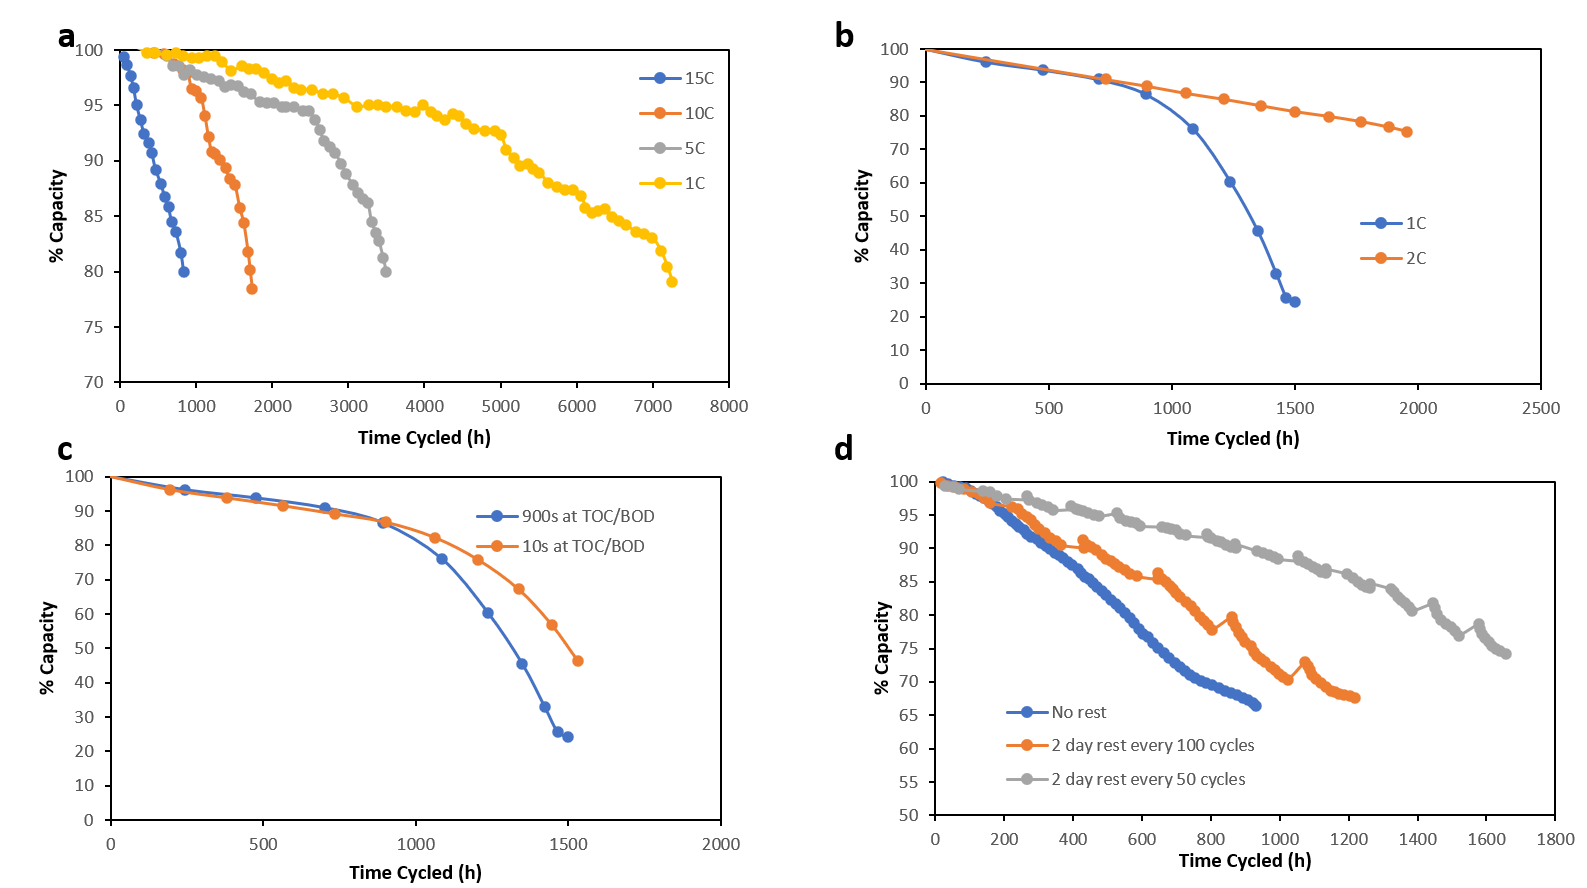
\includegraphics[scale = 0.6]{figures/Discharge-rest_time.png}
\caption{Discharge rate and rest time have mixed effects on knee point onset depending on the testing conditions. Data from Figure \ref{fig:discharge-rest_cycle} replotted with a time-based axis. (a) Higher discharge rate accelerates knee onset. Adapted from \cite{omar_lithium_2014} (b) Lower discharge rate accelerates knee onset. Adapted from \cite{keil_linear_2019} (c) Longer rest time accelerates knee onset. Adapted from \cite{keil_linear_2019} (d) Shorter rest time accelerates knee onset. Adapted from \cite{epding_investigation_2019}.}
\label{fig:discharge-rest_time}
\end{figure}

% \bibliographystyle{myIEEEtran}
\bibliography{refs_zotero}

\end{document}